\documentclass[12pt, a4paper]{report}
% for guidance, see phd_work/mnras_guide.pdf
%\setlength\parindent{0pt}

\usepackage[english]{babel}
\usepackage[utf8x]{inputenc}
\usepackage[T1]{fontenc}

%\documentclass[useAMS,usenatbib]{mn2e}
\newcommand{\aap}{A\&A}
\newcommand{\araa}{ARAA}
\newcommand{\mnras}{MNRAS}
\newcommand{\apjl}{ApJL}
\newcommand{\apjs}{ApJS}
\newcommand{\apj}{ApJ}
\newcommand{\aj}{ApJ}
\newcommand{\nat}{Nature}
\newcommand{\pasa}{PASA}
\newcommand{\pasj}{PASJ}
\newcommand{\pasp}{PASP}
\newcommand{\aapr}{A\&AR}
\newcommand{\procspie}{Proc. SPIE}
\newcommand{\apss}{Ap\&SS}
%\newcommand{\rsquo}{`}

\usepackage{graphicx}
%\usepackage{braket}
\usepackage[english]{babel}
\usepackage{upgreek}
\usepackage{graphicx}
\usepackage{float}
\usepackage{natbib}
\usepackage{amsmath}
\usepackage{amssymb}
\usepackage{tabularx,ragged2e,booktabs,caption}
\usepackage{graphicx} % for images
\usepackage[font=small]{caption}
\usepackage{setspace}
\usepackage{epstopdf}
\usepackage{subcaption}


% ALW edit: FORMAT FOR INCLUDING PDF IMAGES!!!
% for guidance, see phd_work/grfguide.pdf
%\includegraphics[<options>]{filename.pdf}


%%%%%%%%%%%	Page layout settings that follow JMU regulations     %%%%%%%%%%

\setlength{\hoffset}{0mm}
\setlength{\oddsidemargin}{0mm}
\setlength{\evensidemargin}{0mm}

\setlength{\voffset}{-10mm}
\setlength{\topmargin}{0mm}
\setlength{\headheight}{10mm}
\setlength{\headsep}{10mm}

\setlength{\textheight}{220mm}
\setlength{\textwidth}{155mm}

\setlength{\columnsep}{10mm}
\setlength{\marginparsep}{0mm}
\setlength{\marginparwidth}{0mm}
\setlength{\footskip}{20mm}

\setlength{\parindent}{0.3in} % Size of indent at the start of a new paragraph - originally 0.0in
\setlength{\parskip}{0.0in} % Spacing between paragraphs - originally 0.1in

\usepackage[hang,splitrule]{footmisc}

\addtolength{\footskip}{0.5cm}
\setlength{\footnotemargin}{0.3cm}
\setlength{\footnotesep}{0.4cm}

\makeatletter
\let\splitfootnoterule=\pagefootnoterule
\makeatother

%%%%%%%%%%%%%%%%%%%         Title Page            %%%%%%%%%%%%%%%%%%%%
\pagestyle{headings}

\begin{document}
\begin{titlepage}
\pagenumbering{arabic}

\vspace*{-0.4cm}

\begin{center}
\hrule
\vspace*{0.5cm}
{\Huge \sc Modelling extinction in stellar populations \par}
\vspace*{0.5cm}
\hrule

\vspace*{5mm}
{\normalsize M.Phil. thesis}

\vfill

{\bf Alexander Lisboa-Wright}

\end{center}

\vspace*{1.0cm}

\hrule
\vspace*{0.2cm}
\centering{Astrophysics Research Institute, Liverpool John Moores University}\\
\centering{September 2018}

\end{titlepage}

\begin{abstract}
\end{abstract}

\chapter{Units and terminology}
Unless stated otherwise, all quantities will be described in CGS units (masses in grams, lengths in centimetres, times in seconds, energies in ergs). \\*
\begin{tabular}{r@{ }c@{ }l}
$M$ &:& mass\\
$M_{\odot} = 1.989 \times 10^{33} \textnormal{ g}$ &:& solar mass\\
$L$ &:& luminosity\\
$L_{\odot} = 3.842 \times 10^{33} \textnormal{ erg s}^{-1}$ &:& solar luminosity\\
$g$ &:& gravity\\
$R$ &:& radius\\
$G = 6.6723 \times 10^{-8} \textnormal{ cm}^{3} \textnormal{ g}^{-1} \textnormal{ s}^{-2}$ &:& gravitational constant\\
$\sigma_{\textnormal{SB}} = 5.678 \times 10^{-5} \textnormal{ erg cm}^{-2} \textnormal{ K}^{-4} \textnormal{ s}^{-1}$ & : & Stefan-Boltzmann constant\\
\end{tabular}
\\*
$M$ : mass\\*
$M_{\odot} = 1.989 \times 10^{33} \textnormal{ g}$ : solar mass\\*
$L$ : luminosity\\*
$L_{\odot} = 3.842 \times 10^{33} \textnormal{ erg s}^{-1}$ : solar luminosity\\*
$g$ : gravity\\*
$R$ : radius\\*
$G = 6.6723 \times 10^{-8} \textnormal{ cm}^{3} \textnormal{ g}^{-1} \textnormal{ s}^{-2}$ : gravitational constant\\*
$\sigma_{\textnormal{SB}} = 5.678 \times 10^{-5} \textnormal{ erg cm}^{-2} \textnormal{ K}^{-4} \textnormal{ s}^{-1}$ : Stefan-Boltzmann constant\\*


\chapter{Introduction}
\section{Motivation}
As the light emitted from a star travels towards a distant observer, its intensity, or flux, $F$ decreases with distance $d$ via an inverse-square law:

\begin{equation}
\label{flux_def}
F = \frac{L}{4 \pi d^{2}}
\end{equation}

where $L$ is the star's luminosity, which is an intrinsic property of the star (i.e., independent of the observer). Equation \ref{flux_def} is a natural consequence of the same light wave expanding outwards from its source into a progressively larger spherical volume of empty space.
However, the interstellar medium is not a perfect vacuum. It contains many different structures, such as diffuse gas clouds, that can absorb or scatter light passing through, depending on the wavelength of the incoming photons, the spacing between the individual atoms (i.e.,the density of the medium) and the quantum levels in the atoms occupied by their electrons. These absorption and scattering events are known as interstellar extinction. For a given source, its interstellar extinction coefficient represents the sum of the effects of all extinction events along the line-of-sight between the source and the observer.
Interstellar extinction preferentially affects light at shorter (i.e., bluer) wavelengths. Therefore, the effect of extinction is sometimes referred to as ``reddening'', despite the fact that this term is also applied to a related, but distinct, quantity (see Section \ref{extinc_desc}).

\section{Observational constraints}
No telescope can view the sky at all spectral wavelengths - it would be wholly impractical due to the sheer number of sources across the spectrum, as well as the fact that telescope resolution depends on the wavelength of the incoming light. Therefore, modern telescopes are equipped with a system of filters or bands, which allow only light within a narrow range of wavelengths. In a filter system, the individual filters are designed to operate best at different wavelengths. The system will be therefore have the following properties:

\begin{itemize}
\item the filters cover a much wider range of spectral wavelengths when combined than a single filter would alone; this is used to observe sources at different wavelengths to determine its spectral colour ** (see Section ***).
\item 
\end{itemize}

Filters - Johnson, ACS, WFC/UVIS, Gaia
In this project, three broad-band filter systems were employed. These are the Advanced Camera for Surveys (ACS) and the Ultraviolet Imaging Spectrograph channel of the Wide-Field Camera 3 (WFC3/UVIS), both mounted on the Hubble Space Telescope (HST), and the single filter set mounted on the Gaia space observatory.

ACS was installed on HST in 2002 and repaired in 2009, when WFC3 was also installed.

\begin{table}
\begin{center}
\begin{tabular}{cccccc}
\hline
System & Filter & Peak wavelength / \AA & FWHM / \AA \\
\hline

& F435W & 4760 & 729 \\
& F475W & 5000 & 986 \\
& F555W & 5060 & 841 \\
ACS & F606W & 6690 & 1566 \\
& F625W & 6480 & 978 \\
& F775W & 7320 & 1017 \\
& F814W & 7460 & 1657 \\
\hline
& F218W & 2175 & 300 \\
& F225W & 2250 & 500 \\
& F275W & 2750 & 500 \\
& F300X &  & 2775 \\
& F336W & 3375 & 550 \\
& F390W & 3900 & 1000 \\
WFC3 & F438W & 4320 & 695 \\
& F475W & 4750 & 1520 \\
& F555W & 5410 & 1605 \\
& F606W & 5956 & 2340 \\
& F625W & 6250 & 1550 \\
& F775W & 7760 & 1470 \\
& F814W & 8353 & 2555 \\
\hline
& G &  &  \\
Gaia & G\textsubscript{bp} &  &  \\
& G\textsubscript{rp} &  &  \\
\hline

\end{tabular}
\caption{Basic properties of the filters employed in this project}
\label{filter_basics}
\end{center}
\end{table}

Filters thus*** present a challenge when trying to determine stellar spectra acccurately. This task is further complicated by the fact that, even in the wavelength range where a filter does detect incoming flux, the fraction of light it detects, known as the transmittance, is not uniform across the range. The transmittance as a function of wavelength is known as a transmission curve, bandpass or filter response function. Examples of response functions for some**** of the filters employed in this project are shown in Figure \ref{ACS_response_funcs}. By comparing these with the filters' information in Table \ref{filter_basics}, it can be seen that the exact shape of the response function could have a significant impact on the observed spectrum if not taken into account.
The values in the column labelled 'FWHM' represents the full width at half-maximum. In this case, it is defined as the difference between the lowest and highest wavelength values at which the transmittance value is half of its maximum value for the filter, typically assuming the response function can be approximated as a Gaussian distribution. The FWHM acts as a proxy*** for the wavelength range within which the filter can reliably be used for observations.

The wavelengths of light visible to an average human eye are in the range 3800-7400 \AA . Hence, the filters used here cover wavelengths from the soft-ultraviolet (soft-UV) to the near-infrared (NIR),  including all visible wavelengths.

\begin{figure}[h]
\begin{center}
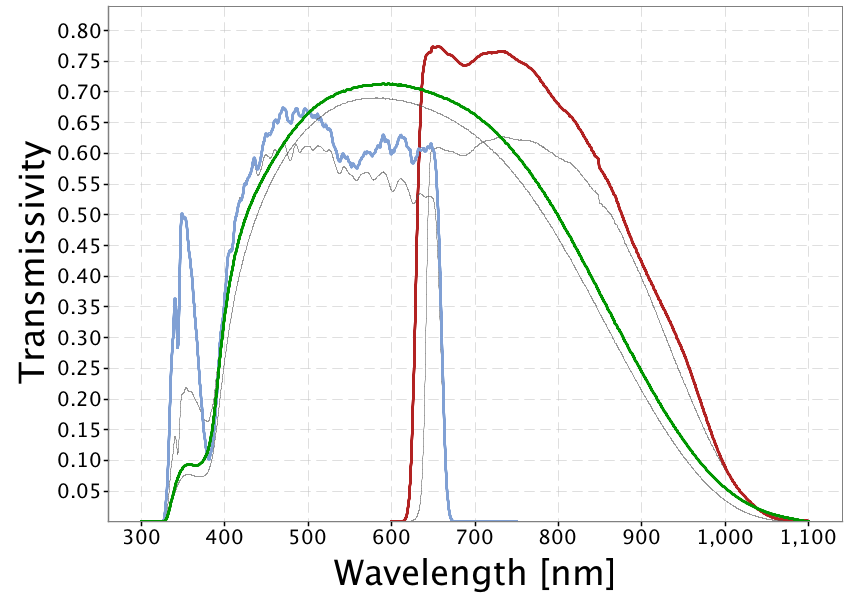
\includegraphics[scale=0.5]{GaiaDR2Passbands.png}
\caption{Filter response functions for Gaia photometric filters.} %Source: https://www.cosmos.esa.int/web/gaia/iow_20180316}
\label{ACS_response_funcs}
\end{center}
\end{figure}

\begin{figure}[h]
\begin{center}
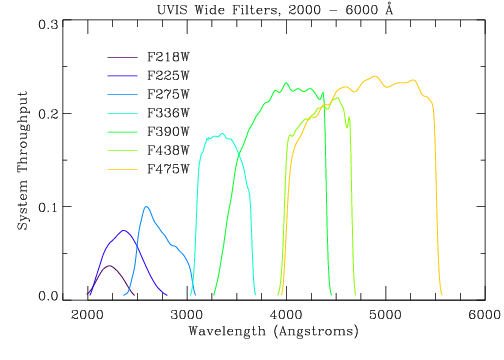
\includegraphics[scale=0.5]{UVIS_Wide1.jpg}
\caption{Filter response functions for wide-field WFC3 filters.} %Source: http://www.stsci.edu/hst/wfc3/ins_performance/throughputs/UVIS_filterthru.html}
\label{WFC3_response_funcs1}
\end{center}
\end{figure}

\begin{figure}[h]
\begin{center}
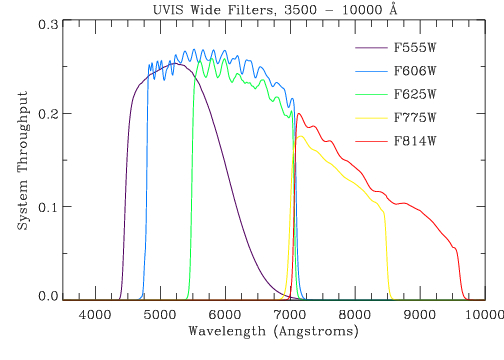
\includegraphics[scale=0.5]{UVIS_Wide2.jpg}
\caption{Filter response functions for wide-field WFC3 filters.} %Source: http://www.stsci.edu/hst/wfc3/ins_performance/throughputs/UVIS_filterthru.html}
\label{WFC3_response_funcs2}
\end{center}
\end{figure}

\begin{figure}[h]
\begin{center}
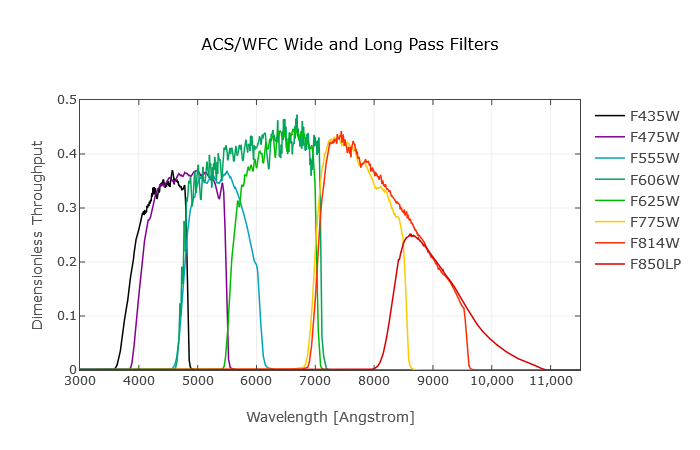
\includegraphics[scale=0.5]{ACS_Wide.png}
\caption{Filter response functions for wide-field ACS filters. Source: http://www.stsci.edu/hst/acs/analysis/throughputs}
\label{ACS_response_funcs}
\end{center}
\end{figure}

\section{Basics of stellar evolution} \label{stel_evol}
In the main sequence, nuclear fusion occurs in the core and any products must be subjected to mixing effects to reach the atmosphere. Since stellar interiors are physically fluid, heavier nuclei, which are denser, preferentially gather in regions close to the star's centre of gravity. Therefore, processes such as convection, thermohaline mixing and radiative levitation would be needed to induce a noticeable change in surface composition. However, these processes require certain physical conditions on local scales, if they are to be sustained. 

****On the main-sequence, only low-mass stars ($M_{*} \lesssim 0.5M_{\odot}$) have fully-convective interiors. Massive ($M_{*} \gtrsim 1.5M_{\odot}$) stars have convective cores, but radiative envelopes. Intermediate-mass stars, including the Sun, have radiative cores and convective envelopes. Since regions in which energy transport is dominated by radiative effects.

\begin{equation}
\nabla_{\textnormal{rad}} = \frac{3\kappa LP}{16\pi acGmT^{4}}
\end{equation}

To illustrate, let us consider a bubble of gaseous material in pressure-equilibrium with its surroundings and represent mixing as a significant change in the bubble's (radial) position on a significant time-scale, arising from small differences in the remaining 3 thermodynamic quantities between the bubble and its surroundings. For a non-rotating star, using a simple linear approach, together with the Archimedes principle, gives a set of 4 homogeneous differential equations for the (small) differences in $P$, $T$, $\mu$ and $r$ (Equations (3.1)-(3.4) in \cite{2017RSOS....470192S}). If $\Delta x_{i}$ are the differences in the 4 parameters, taking the ansatz form $\Delta x_{i} = B_{i} e^{nt}$ allows for a solution as a 3rd-order polynomial in $n$ (Equation (3.5) in \cite{2017RSOS....470192S}), if the determinant of the relevant matrix (dependent of the values of the $B_{i}$) is zero. The Routh-Hurwitz stability criterion can then be applied to this polynomial to give a general solution for $n$. For a physically-unstable solution, the exponent in the $\Delta x_{i}$ equation must be positive, i.e. $n$ must satisfy the condition $\operatorname{Re}(n) > 0$. Hence, the subsequent constraints on the polynomial coefficients form all the possible conditions for instability,  of which at least one must be satisfied. These constraints take the following form:

\begin{align}
\nabla _{\mu} &< 0 \label{mu_inv_ineq} \\
\nabla _{\textnormal{rad}} &> \nabla _{\textnormal{ad}} \label{schwarz_ineq} \\
\nabla _{\textnormal{rad}} &> \nabla _{\textnormal{ad}} + \left( \frac{\phi}{\delta} \right) \nabla _{\mu} \label{ledoux_ineq}
\end{align}

where $\nabla _{\mu} = d\ln\mu / d\ln P$, $\nabla _{\textnormal{rad}} = \left(\partial\ln T / \partial\ln P \right)_{\textnormal{rad}}$ and $\nabla _{\textnormal{ad}} = \left(\partial\ln T / \partial\ln P \right)_{\textnormal{ad}}$ are the temperature-pressure gradients for the local environment (dominated by radiation pressure) and the bubble (treated as an adiabatic ideal gas), respectively, $\phi = \left( \partial \ln\rho / \partial \ln\mu \right)_{P,T}$ and $\delta = -\left( \partial \ln\rho / \partial \ln T \right)_{P,\mu}$  \citep{1980A&A....91..175K}.

\section{Previous studies}
\cite{1989ApJ...345..245C} used observations of bright main-sequence stars to produce empirical equations describing the ratio of extinction coefficients in a chosen filter $X$ ($A_{X}$) and the Johnson-$V$ filter ($A_{V}$), respectively. From this point onward, this ratio will be referred to as $A_{X}/A_{V}$. ****They produced a basic universal equation of the form:

% avoided the complications of using reddening (which is not itself intrinsic and whose implications be impacted by the choice of filters) by 

\begin{equation}
A_{\lambda}/A_{V} = a(x) + b(x)/R_{V},
\label{CCM_general}
\end{equation}

where $x \equiv 1/\lambda$ and $R_{V} \equiv A(V)/E(B-V)$. The total wavelength range was divided into 4 subranges, each with a governing pair of empirically-determined equations (to determine $a(x)$ and $b(x)$, respectively). The CCM89 model underpins more recent studies of intrinsic effects on extinction (\cite{2008PASP..120..583G}, \cite{2018MNRAS.479L.102C}), and provides the basis for the synthetic $A_{X}/A_{V}$ dataset in this project.
\cite{2008PASP..120..583G} produced data tables of bolometric corrections for stellar atmosphere models with parameters Teff, log(g), [Fe/H]****.

***Casagrande \& Vandenberg (2014, 2018a, 2018b)



\chapter{Theory}
\section{Extinction definition} \label{extinc_desc}
Extinction is defined using the standard astronomical system of flux magnitudes. In general, the difference between two flux measurements, $F_{1}$ and $F_{2}$, in magnitudes, is expressed as:
\begin{equation}
\label{mags_def}
m_{1} - m_{2} = -2.5\log \left( \frac{F_{1}}{F_{2}} \right)
\end{equation}

where $m_{1}$ and $m_{2}$ are the magnitudes for $F_{1}$ and $F_{2}$, respectively. However, the flux of a source varies naturally with the distance to the observer (see Equation \ref{flux_def}). To account for this, the distances to the nearest stars was determined independently of their flux, by their parallax from Earth. The parallax $p$ of an object is defined by the angular distance the object moves relative to the ``fixed'' background as the Earth moves a distance of 1AU (the average separation of the Sun and Earth during one complete orbit) perpendicular to the line-of-sight. This allows the distance, $d$, to be measured using the geometry of triangles, combined with the small-angle approximation, as:

\begin{equation}
d/\textnormal{pc} = \frac{1}{(p/\textnormal{arcsec})}
\end{equation}

This gives each astronomical object two fundamental flux measurements. These are the apparent magnitude, $m$, and the absolute magnitude, $M$. The apparent magnitude is the flux magnitude of a source, as observed by the telescope. The absolute magnitude is the projected flux magnitude of the same source if it were to be placed at a distance of 10 parsecs (pc) from the telescope, thus accounting for the distances The relation between these quantities if there is zero extinction can be found by combining Equations \ref{flux_def} and \ref{mags_def}:
% In general, the extinction coefficient $A$ is defined relative to two ubiquitous astrophysical quantities.
\begin{equation}
\label{distance_modulus}
m - M = -2.5\log \left( \left(\frac{10\textnormal{pc}}{d}\right)^{2} \right) = 5\log\left(\frac{d}{\textnormal{pc}}\right) - 5
\end{equation}

The quantity ($m - M$) is known as the distance modulus. It is particularly useful for observing stellar populations, as stars within a single-age population are easily classified using their position on the theoretical Hertzsprung-Russell (HR) diagram or ***some of its observational equivalents, known as colour-magnitude diagrams (CMDs). In the HR diagram, stars of a given age and metallicity are plotted in the luminosity-effective temperature ($L-T_{\textnormal{eff}}$) plane. An example of a HR diagram is shown in Figure ****. It can be seen that all stars lie on a single, complicated line, known as an isochrone. Isochrones for different population ages and metallicities are calculated using theoretical stellar models for the largest possible spread of initial stellar masses. An isochrone in the HR diagram has a number of distinct features:
\begin{itemize}
\item Most stars, including the coolest and least-luminous ones, follow a tight pattern of luminoaity increasing with temperature. This is known as the main sequence (MS)
\item This pattern stops as the luminosity continues to increase slowly but with decreasing temperature. The end of the MS is called the main-sequence turn-off (MSTO), which is followed by the sub-giant branch (SGB).
\item After the SGB, the gradient becomes much steeper, with temperate decreasing and luminosity rapidly increasing. This is the red-giant branch (RGB).
\item At the tip of the RGB, stars start becoming fainter and their temperatures increase. Eventually, their is a sequence of stars with near-constant luminosity but a range of effective temperatures. This is the horizontal branch (HB).
\item After the horizontal branch, there is again a rapid increase in luminosity accompanied by a slow decrease in temperature. This is the asymptotic giant branch (AGB).
\end{itemize}

It should be noted that the distance modulus in Equation \ref{distance_modulus} does not include extinction. To link the apparent magnitude to extinction, it is necessary to separate the distance modulus from the observed apparent magnitude, $m_{\textnormal{obs}}$. This can be done by defining the intrinsic apparent magnitude, $m_{0}$, such that:

\begin{equation}
\label{intrinsic_app_mag}
m_{0} - M = 5\log(d/\textnormal{pc}) - 5
\end{equation}

i.e., the distance modulus is solely dependent on the distance to the  sources. Therefore, the extinction $A$ can be defined as:

\begin{equation}
\label{bol_extinc}
A = m_{\textnormal{obs}} - m_{0}
\end{equation}

This fits with the definition of interstellar extinction given earlier, i.e. as the flux lost solely due to scattering and absorption in the interstellar medium.

However, as noted earlier, in astronomy it is infeasible to attempt observations by a single instrument at all wavelengths. Telescopes instead are generally purpose-built to study a single, relatively narrow wavelength range of the EM spectrum. Within this range, telescope observation ranges are further divided by filters or passbands, one of which is placed on their aperture at any given observation time****. As shown in Figure \ref{ACS_response_funcs}, \ref{WFC3_response_funcs1}, \ref{WFC3_response_funcs2} and****, a single generic filter $X$ has a range of wavelengths for which it is able to detect flux. It can also be seen in these figures that the transmittance of the filter changes as a function of wavelength

\begin{equation}
f_{\lambda} = \frac{2hc}{\lambda^{5}\left(\exp\left({\frac{hc}{\lambda k_{B}T}}\right) - 1\right)}
\label{planck_bb}
\end{equation} 

****In this project, when comparing effects of different extinction treatments and, subsequently, when comparing observational datasets (with uncertainties in the values of their objects' stellar parameters and unknown extinction coefficients) to theoretical datasets via color-magnitude diagrams (CMDs), the most convenient format is to add the (theoretical) extinction coefficients to the theoretical dataset magnitudes (i.e., absolute magnitudes). As a result, the quantity from each dataset that is being compared in the CMDs is the absolute magnitude plus an extinction coefficient. If we label this quantity $M_{\textnormal{ext},X}$, we can define it bolometric as:

\begin{equation}
M_{\textnormal{ext},X} = M_{X} + A_{X}
\end{equation}

To measure a star's effective temperature, observers compare the star's observed flux in two filters at different wavelengths, typically in the UV-IR wavelength range. This is because a star with a higher effective temperature will be more luminous in every filter than a cooler star at the same position. This creates uncertainty if the distance measurement cannot be obtained independent of photometry.

\section{Bolometric corrections} \label{BC_theory}
All the equations in Section ****, including those for extinction, are not useful when applied to telescopes, as any filter will only detect a small fraction of the stellar flux across all wavelengths (known as the bolometric stellar flux) that reaches the telescope. The missing information resulting from this observational constraint renders it difficult to determine the interstellar extinction. These constraints much be mitigated before an accurate value of the extinction coefficient can be determined. This mitigation is carried out by employing bolometric corrections.

The use of bolometric corrections requires the detailed knowledge of stellar spectra least susceptible to significant extinction, i.e., nearby stars with high apparent fluxes. Only with complete knowledge of the spectrum from a reference star can the true spectrum of a distant star with unknown extinction be calculated. The spectra of these stars can be computed by using a grid of predicted fluxes from a stellar atmosphere model, the grid being composed of the stellar parameters known to change emission in stellar atmospheres. These are effective temperature, surface gravity and metallicity. For all filter systems studied in this project, the nearby star Vega ($\alpha$ Lyr) was used as the reference object. Using Vega as the reference star is the most well-known approach to calibration \citep{2014MNRAS.444..392C}

The effective temperature ($T_{\textnormal{eff}}$) of a star is defined as the temperature of a black body which produces the closest matching bolometric spectrum to that of the star. This approximation is valid because all stars have been observed to have spectra that closely resemble those of black bodies, with the notable exception of atmospheric absorption lines.
\begin{equation}
L = 4 \pi R^{2} \sigma_{SB} T_{\textnormal{eff}}^{4}
\label{Teff_def}
\end{equation}
Effective temperature has an effect on interstellar extinction due to its strong effect on the stellar luminosity and, hence, the flux. For a higher flux, more photons are likely to interact with the ISM, hence a higher extinction coefficient.

The metallicity of a star is defined as the fractional abundance of heavy elements, often approximated by iron alone, relative to the star's hydrogen abundance, compared to that of the Sun. The abundances are determined by the strength of the elements' characteristic atomic absorption lines in the stellar spectra.

\begin{equation}
\textnormal{[Fe/H]} = \log(N_{\textnormal{Fe}}/N_{\textnormal{H}}) - \log(N_{\textnormal{Fe},\odot}/N_{\textnormal{H},\odot})
\label{FeH_def}
\end{equation}

Since the output is logarithmic, a value of [Fe/H] = 0 indicates solar metallicity. An increase in metallicity would cause the corresponding absorption lines to be stronger, thus reducing the observable flux.

The definition of the stellar surface gravity $g$ is simply the value of the standard Newtonian gravtitional acceleration, applied to the stellar surface (the mass is the total stellar mass, $M_{*}$, and the distance is the stellar radius, $R_{*}$):

\begin{equation}
g = \frac{GM_{*}}{R_{*}^{2}}
\label{gravity_def}
\end{equation}

A higher surface gravity represents a surface with a higher atomic number density. This environment produces a shorter mean free path for photons overall, meaning a smaller collision timescale. If the timescale is sufficiently small, the limit provided by Heisenberg's Uncertainty Principle causes an increase in the uncertainty of the energy absorbed by the atomic electron during the interaction with the photon:

\begin{equation}
\Delta E \Delta t \geq \hbar/2
\label{heisenberg}
\end{equation}

This effect, known as ``pressure broadening'', causes a symmetrical distribution of absorption energies (and wavelengths) about the normal emission energy for that particular atomic state. This means fewer photons pass through the surface, thereby reducing the surface flux.

After accounting for a general extinction effect on an object's emission, its apparent magnitude in a given filter $X$ (i.e. wavelength range, which we define as increasing from $\lambda _{1}$ to $\lambda _{2}$) is given by:

\begin{equation}
m_{X} = -2.5 \log_{10} \left(\frac{ \int_{\lambda_{1}}^{\lambda_{2}} f_{\lambda} \left( 10^{-0.4 A_{X,\lambda}} \right) S_{\lambda} d\lambda }{ \int_{\lambda_{1}}^{\lambda_{2}} f_{\lambda}^{0} S_{\lambda} d\lambda }\right) + m_{X}^{0}
\label{app_mag_def}
\end{equation}

where $f_{\lambda}$ represents the monochromatic flux at a given wavelength $\lambda$ at the observer distance, $A_{X,\lambda}$ is the extinction value as a function of wavelength, $S_{\lambda}$ represents the filter response function and $f_{\lambda}^{0}$ and $m_{X}^{0}$ represent the monochromatic flux and apparent magnitude, respectively, of a known reference object in $X$.

%Since our goal, ultimately, is to document potential effects of fundamental stellar properties upon observables, we need to connect the observational and idealised scenarios, for which we use bolometric corrections.

To derive the equation linking a bolometric correction with the extinction parameter, we start with the definition of a bolometric correction in a filter $X$, which is denoted by $BC_{X}$:

\begin{equation}
BC_{X} \equiv M_{\textnormal{bol}} - M_{X}
\label{BC_def}
\end{equation}

where $M_{X}$ is the absolute magnitude of the object in $X$ and $M_{\textnormal{bol}}$ is its (predicted) absolute bolometric magnitude, defined relative to the Sun using:

\begin{equation}
M_{\textnormal{bol}} = M_{\textnormal{bol},\odot} - 2.5 \log_{10} \left( \frac{4\pi R^{2}F_{\textnormal{bol}}}{L_{\odot}} \right)
\label{mbol_sun}
\end{equation}

where  $F_{\textnormal{bol}}$ is the bolometric stellar flux at its surface, $R$ is the stellar radius, $M_{\textnormal{bol},\odot}$ is the solar absolute bolometric magnitude, which is assumed in this work to have a value of 4.75 and $L_{\odot}$ is the solar luminosity, for which a value of $3.844 \times 10^{33}$ erg s$^{-1}$ is used. Bolometric corrections can be expressed as a function of extinction using the universal definition of $M_{X}$ in terms of $m_{X}$ and the distance $d$ to the source:

\begin{equation}
M_{X} = m_{X} - 2.5 \log_{10}\left( \left( \frac{d}{10 \textnormal{pc}} \right)^{2} \right),
\label{abs_mag_def}
\end{equation}

together with the equation $f_{\lambda}d^{2}=F_{\lambda}R^{2}$, where $F_{\lambda}$ is the monochromatic flux at $\lambda$ at the stellar surface. This gives the final function for a bolometric correction for filter $X$:

\begin{align}
\begin{split}
BC_{X} &= M_{\textnormal{bol},\odot} - m_{X}^{0} - 2.5 \log_{10} \left( \frac{4\pi R^{2}F_{\textnormal{bol}}}{L_{\odot}} \right) \\
&+ 2.5 \log_{10} \left( \frac{\int_{\lambda_{1}}^{\lambda_{2}} F_{\lambda} \left( 10^{-0.4 A_{X,\lambda}} \right) S_{\lambda} d\lambda}{\int_{\lambda_{1}}^{\lambda_{2}} f_{\lambda}^{0} S_{\lambda} d\lambda} \right)
\label{BC_extinc}
\end{split}
\end{align}

For a filter $X$, the extinction parameter $A_{X} = A_{X,\lambda}$ must be calibrated relative to a known value. In this work we will input a value of the extinction in the well-studied Johnson-$V$ filter, $A_{V}$. To extract $A_{X}$, we use the simple relation:

\begin{equation}
A_{X} = \left( \frac{A_{X}}{A_{V}} \right) A_{V}
\label{ratio_eq}
\end{equation}

together with the chosen value of $A_{V}$ (for this project the values were $A_{V} =$ 0, 1 - note that $BC_{X}(A_{V}=0)$ effectively assumes no extinction), before taking the difference between the two $BC_{X}(A_{V})$, giving the following equation:

\begin{align}
\begin{split}
BC_{X}(0) - BC_{X}(A_{V}) &= 2.5 \log_{10} \left( \frac{\int_{\lambda_{1}}^{\lambda_{2}} F_{\lambda}  S_{\lambda} d\lambda}{\int_{\lambda_{1}}^{\lambda_{2}} F_{\lambda}\left( 10^{-0.4 \left(A_{X,\lambda}/A_{V}\right)A_{V}} \right) S_{\lambda} d\lambda} \right)
\\ &\approx \left(A_{X}/A_{V}\right)A_{V}
\label{BCs_diff}
\end{split}
\end{align}

****average over the wavelength interval $[\lambda_{1},\lambda_{2}]$ which is a valid assumption \citep{2014MNRAS.444..392C}, as the CCM relations, which were derived using data from stars observed in the Johnson broad-band filters. Due to the nature of the filters' bandpasses, the CCM relations overestimate the extinction in the near-IR and blue-visible Johnson filters
%\citep{1999fitzpatrick.

\chapter{Methodology}
\section{Software used}
The tables of bolometric corrections were generated using a FORTRAN 77 code incorporating the steps described in Section \ref{BC_theory}, inputs with tables describing the response functions of all three filter systems at short**** wavelength intervals and ATLAS9 model atmosphere tables at the same wavelengths, with the number of tables for each stellar metallicity value equal to the total number of (**Teff,, log(g)) combinations available (see Table 1 of \cite{2004astro.ph..5087C} for details of the coverage in Teff-log(g) parameter space).

Once the bolometric correction tables were produced, all subsequent processes were written in Python 2.7.

\begin{table}
\begin{center}
\begin{tabular}{cccc}
\hline
%\multirow{2}{*}{System} & \multirow{2}{*}{Filter} & \multirow{2}{*}{$A_{1}$ function} & \multicolumn{3}{c}{$A_{1}$ coefficients} \\ \cline{4-6}
%\textbf{Filter} \\
Parameter / unit & Minimum & Maximum & Number of values \\
\hline
$T_{\textnormal{eff}}$ / K & 3500 & 50000 & 76 \\
log( $g$ / cm s$^{-2}$) & 0.0 & 5.0 & 11 \\
$\textnormal{[Fe/H]}$ & -2.0 & 0.5 & 4 \\
\hline
\end{tabular}
\caption{Ranges for the input parameters for ATLAS9 atmospheric models}
\label{atlas9_input}
\end{center}
\end{table}


The isochrones used were generated using the latest Bag of Stellar Tricks and Isochrones (BaSTI) web interface \citep{2018ApJ...856..125H}. The filter systems whose throughput data were employed by BaSTI to generate the fluxes for the isochrones were ACS, WFC3 and Gaia-DR2. It should be noted that the WFC3 isochrone output does not include flux magnitudes for the F300X filter.

\section{Finding \& fitting functions}
When calculating the bolometric corrections, the reference values taken by the parameters for Vega were:

\begin{enumerate}
\item $m_{X}^{0} = 0.03$ for the Gaia filters
\item $m_{X}^{0} = 0.00$ for the Hubble WFC3 filters
\end{enumerate}

together with $M_{\textnormal{bol},\odot} = 4.75$. Equation \ref{CCM_general}, with the different wavelength regimes for $a(x)$ and $b(x)$ described by CCM89, was used with the $A_{V}$ calibration values to simulate the extinction parameter in Equation \ref{BC_extinc}. $R_{V}$ was set to a value of 3.1, the standard value for the diffuse interstellar medium. The integration was carried out by iteratively adding the integrand results at regular small wavelength intervals. The non-zero calibration value of $A_{V} = 1$ was chosen, as this allows for significant changes in $A_{X}/A_{V}$ from Equation (\ref{BCs_diff}), while also being close enough to zero to avoid significant changes in $A_{X}/A_{V}$ due to the Forbes effect \citep{2008PASP..120..583G}.

The Forbes effect occurs as a broadband beam of light, such as that passes through an extended partially-transparent medium, such as a series of glass plates, the Earth's atmosphere or an interstellar gas cloud. It states that the greater the distance travelled by a light beam through the medium, the more penetrating the beam becomes \citep{1842RSPT..132..225F}. If we use the case of the glass plates as an example, this means that the fraction of the light incident on the $n$th plate in the series which is separated by that plate from the original path is always greater than the corresponding fraction at the ($n+1$)th plate. The physical basis for the Forbes effect is that those photons in the original beam with wavelengths that make them the most likely to be absorbed or refracted are separated from the beam earlier. Therefore, as the beam travels through the medium, its constituent photons are progressively less likely to be separated. Since a higher fraction of its photons are retained as the distance through the medium increases, the beam is more penetrating.

The Forbes effect thus has an impact on the non-zero $A_{V}$ value used because if a uniform medium is assumed, as here, where $R_{V}$ is held constant at the standard diffuse ISM value of 3.1****, a larger $A_{V}$ value implies a longer path through the ISM, and thus a stronger Forbes effect. According to \cite{2008PASP..120..583G}, any ****significant impact from the Forbes effect on the values of $A_{X}/A_{V}$ occurs for a chosen $A_{V} \gtrsim 5$. Therefore, the choice of $A_{V} = 1$ made for this project should avoid serious problems from the Forbes effect.

****Guesswork!

To generate extinction-coefficient ratios $A_{X}/A_{V}$ from the bolometric correction data

To find usable functions required prioritising which parameters to model first, as increasing the number of stellar parameters would cause an increase in the number of coefficients to fit for the function being tested. This would create a higher risk of degeneracies between coefficients and increase the fitting output errors such that the errors obscure any useful information about the coefficients themselves.

The bolometric flux of a black body can be calculated as the total area under the curve described by the Planck function per unit wavelength/frequency as a function of wavelength/frequency. Since stellar emission spectra can be reasonably approximated by a black body emission with absorption lines, it can be seen from Equation\ref{Teff_def} that the greatest effect on stellar spectra, and therefore on the extinction coefficient, will come from effective temperature. Therefore, the initial functions to be fitted were simple analytical functions of $T_{\textnormal{eff}}$ only:

\begin{equation}
A_{\textnormal{pow}} (T_{\textnormal{eff}}) = a (T_{\textnormal{eff}})^{b} + c
\label{Teff_pow}
\end{equation}

while the second case (denoted by `exp') models an exponential:

\begin{equation}
A_{\textnormal{exp}} (T_{\textnormal{eff}}) = a \exp{(b T_{\textnormal{eff}})} + c
\label{Teff_exp}
\end{equation}

\section{Isochrone data fitting}
To obtain isochrones from the BaSTI online database, the desired age range, initial metallicity and filter system must be specified. Therefore, the values of these quantities are shared by all stellar objects. For the stages in stellar evolution prior to the main-sequence turn-off, any changes in atmospheric metallicity are insignificant, due to the factors discussed in Section \ref{stel_evol}.

The output from the BaSTI database for each model stellar object gives the model's initial mass and current mass (i.e. after a time equal to the isochrone age), together with the logarithms of the stellar luminosity in solar units ($\log_{10}(L/L_{\odot})$) and of the effective temperature in K ($\log_{10}(T_{\textnormal{eff}})$), followed by the absolute magnitudes (with zero extinction) of the object in each filter of the system. To derive the surface gravity $g$, we must combine Equation \ref{Teff_def}, to derive the stellar radius, and Equation \ref{gravity_def}. Equation \ref{gravity_LT_calc} shows the resultant definition of $g$:

\begin{equation}
\label{gravity_LT_calc}
g = \frac{4 \pi G M_{*} \sigma_{\textnormal{SB}} T_{\textnormal{eff}}^{4}}{L_{*}}
\end{equation}

After this had been completed, each object had a co-ordinate in ($T_{\textnormal{eff}}$, log($g$)) parameter space, plus the metallicity of the overall isochrone model. The functions described in Section **** were then applied to the dataset of stellar objects, producing filter magnitudes correct

\begin{table}
\begin{center}
\begin{tabular}{ccccc}
\hline
Isochrone & $T_{\textnormal{eff}}$ & $T_{\textnormal{eff}}$ & $\log(g)$ & $\log(g)$ \\
(Age/Myr , [Fe/H]) & minimum & maximum & minimum & maximum \\
\hline
500,0.002 & 2870 & 9640 & 0.886 & 5.137 \\
1000,0.002 & 2824 & 8035 & 1.608 & 5.184 \\
5000,-1.049 & 3118 & 7112 & 0.456 & 5.318 \\
10000,-1.049 & 3086 & 6412 & 0.286 & 5.332 \\
\hline
\end{tabular}
\caption{Ranges of effective temperature and surface gravities in selected BaSTI isochrones}
\label{variable_ranges}
\end{center}
\end{table}

DR2 Babusiaux data, errors

****However, the filter magnitudes in the photometric data were the original apparent magnitudes, not absolute magnitudes. Therefore, to match the attributes**** of the observational and isochrone datasets, it was necessary to both correct the observational fluxes**** for distance and add extinction to the isochrone data. This produces 


\chapter{Results and discussion}
\section{Extinction coefficient models} \label{coef_models}

\begin{table}
\begin{center}
\begin{tabular}{cccccc}
\hline
%\multirow{2}{*}{System} & \multirow{2}{*}{Filter} & \multirow{2}{*}{$A_{1}$ function} & \multicolumn{3}{c}{$A_{1}$ coefficients} \\ \cline{4-6}
%\textbf{Filter} \\
System & Filter & $A_{1}$ function & & $A_{1}$ coefficients & \\
 & & & $a$ & $b$ & $c$ \\
\hline

& F435W & pow & -(3.381$\pm$0.733)$\times 10^{4}$ & -1.394$\pm$0.026 & 1.040$\pm$0.001 \\
& F475W & pow & -457.6$\pm$64.9 & -0.9000$\pm$0.0172 & 1.247$\pm$0.002 \\
& F555W & pow & -(4.383$\pm$0.871)$\times 10^{3}$ & -1.361$\pm$0.023 & 0.6771$\pm$0.0002 \\
ACS & F606W & pow & -(4.383$\pm$0.871)$\times 10^{3}$ & -1.361$\pm$0.023 & 0.6771$\pm$0.0002 \\
& F625W & pow & -(3.381$\pm$0.733)$\times 10^{4}$ & -1.394$\pm$0.026 & 1.040$\pm$0.001 \\
& F775W & pow & -457.6$\pm$64.9 & -0.9000$\pm$0.0172 & 1.247$\pm$0.002 \\
& F814W & pow & -(4.383$\pm$0.871)$\times 10^{3}$ & -1.361$\pm$0.023 & 0.6771$\pm$0.0002 \\ \hline
% -2.32428259e+02  -1.07634845e-03   2.93338391e+00
% -1.28482746e+02  -1.03094181e-03   2.61038997e+00
% -9.72567775e-01  -3.51770388e-04   2.06004238e+00
% -5.33470924e+05  -1.66350652e+00   2.05158490e+00
% -1.51556105e+04  -1.58229494e+00   1.64765130e+00
% -0.59910717 -0.08070638  1.73786479
% -9.99999999e+04  -1.78304457e+00   1.35186267e+00
% -1.20707226e+05  -1.70657822e+00   1.22045256e+00
% -4.59655266e+05  -1.88059297e+00   1.07985380e+00
% -3.13655088e+05  -1.82928924e+00   9.64793923e-01
% -5.47562323e+05  -2.02950259e+00   8.78683006e-01
% -6.32767059e+03  -1.57627077e+00   6.56703339e-01
% -3.72711692e+03  -1.43145264e+00   6.15752594e-01
% -3.38142759e+04  -1.39444200e+00   1.03998507e+00
% -457.55192948   -0.89995256    1.24675509
% -4.38278161e+03  -1.36062232e+00   6.77129794e-01
& F218W & exp & -232.4$\pm$48.1 & -(1.076$\pm$0.043)$\times 10^{-3}$ & 2.933$\pm$0.007 \\
& F225W & exp & -128.5$\pm$13.8 & -(1.031$\pm$0.022)$\times 10^{-3}$ & 2.610$\pm$0.003 \\
& F275W & exp & 0.9726$\pm$0.0581 & -(3.518$\pm$0.109)$\times 10^{-4}$ & 2.060$\pm$0.001 \\
& F300X & pow & -(5.335$\pm$0.936)$\times 10^{5}$ & -1.664$\pm$0.021 & 2.052$\pm$0.001 \\
& F336W & pow & -(1.516$\pm$0.723)$\times 10^{4}$ & -1.582$\pm$0.056 & 1.648$\pm$0.001 \\
& F390W & pow & -0.5991$\pm$0.1494 & -0.08071$\pm$0.09090 & 1.738$\pm$0.309 \\
WFC3 & F438W & pow & -(1.000$\pm$0.463)$\times 10^{5}$ & -1.783$\pm$0.054 & 1.352$\pm$0.001 \\
& F475W & pow & -(1.207$\pm$0.379)$\times 10^{5}$ & -1.707$\pm$0.037 & 1.220$\pm$0.001 \\
& F555W & pow & -(4.560$\pm$1.490)$\times 10^{5}$ & -1.881$\pm$0.038 & 1.080$\pm$0.001 \\
& F606W & pow & -(3.137$\pm$0.911)$\times 10^{5}$ & -1.829$\pm$0.034 & 0.9648$\pm$0.0003 \\
& F625W & pow & -(5.476$\pm$3.709)$\times 10^{5}$ & -2.030$\pm$0.079 & 0.8787$\pm$0.0002 \\
& F775W & pow & -(6.328$\pm$4.571)$\times 10^{3}$ & -1.576$\pm$0.085 & 0.6567$\pm$0.0001 \\
& F814W & pow & -(3.727$\pm$1.381)$\times 10^{3}$ & -1.431$\pm$0.044 & 0.6158$\pm$0.0002 \\ \hline

& G & pow & -(3.381$\pm$0.733)$\times 10^{4}$ & -1.394$\pm$0.026 & 1.040$\pm$0.001 \\
Gaia & G\textsubscript{bp} & pow & -457.6$\pm$64.9 & -0.9000$\pm$0.0172 & 1.247$\pm$0.002 \\
& G\textsubscript{rp} & pow & -(4.383$\pm$0.871)$\times 10^{3}$ & -1.361$\pm$0.023 & 0.6771$\pm$0.0002 \\ \hline

\end{tabular}
\caption{Coefficient values produced by $A_{1}$ fitting}
\label{simpfunc_coeffs_table}
\end{center}
\end{table}

It should be noted that the 

\section{Effect on isochrones}
Given the large number of filters studied in Section \ref{coef_models}, four commonly-used CMD axes were selected to test for any effects of a function-derived $A_{X}$. Two of these are specific to the WFC3 system, with one CMD each for ACS and Gaia.
\subsection{ACS} \label{ACS_isoc}

The CMD chosen for the ACS was the F435W-(F435W-F814W) axis combination. This CMD is useful as it pairs the bluest and reddest wide-field filters for the ACS, which produces larger spectral colours.****

\begin{figure}[h]
\begin{center}
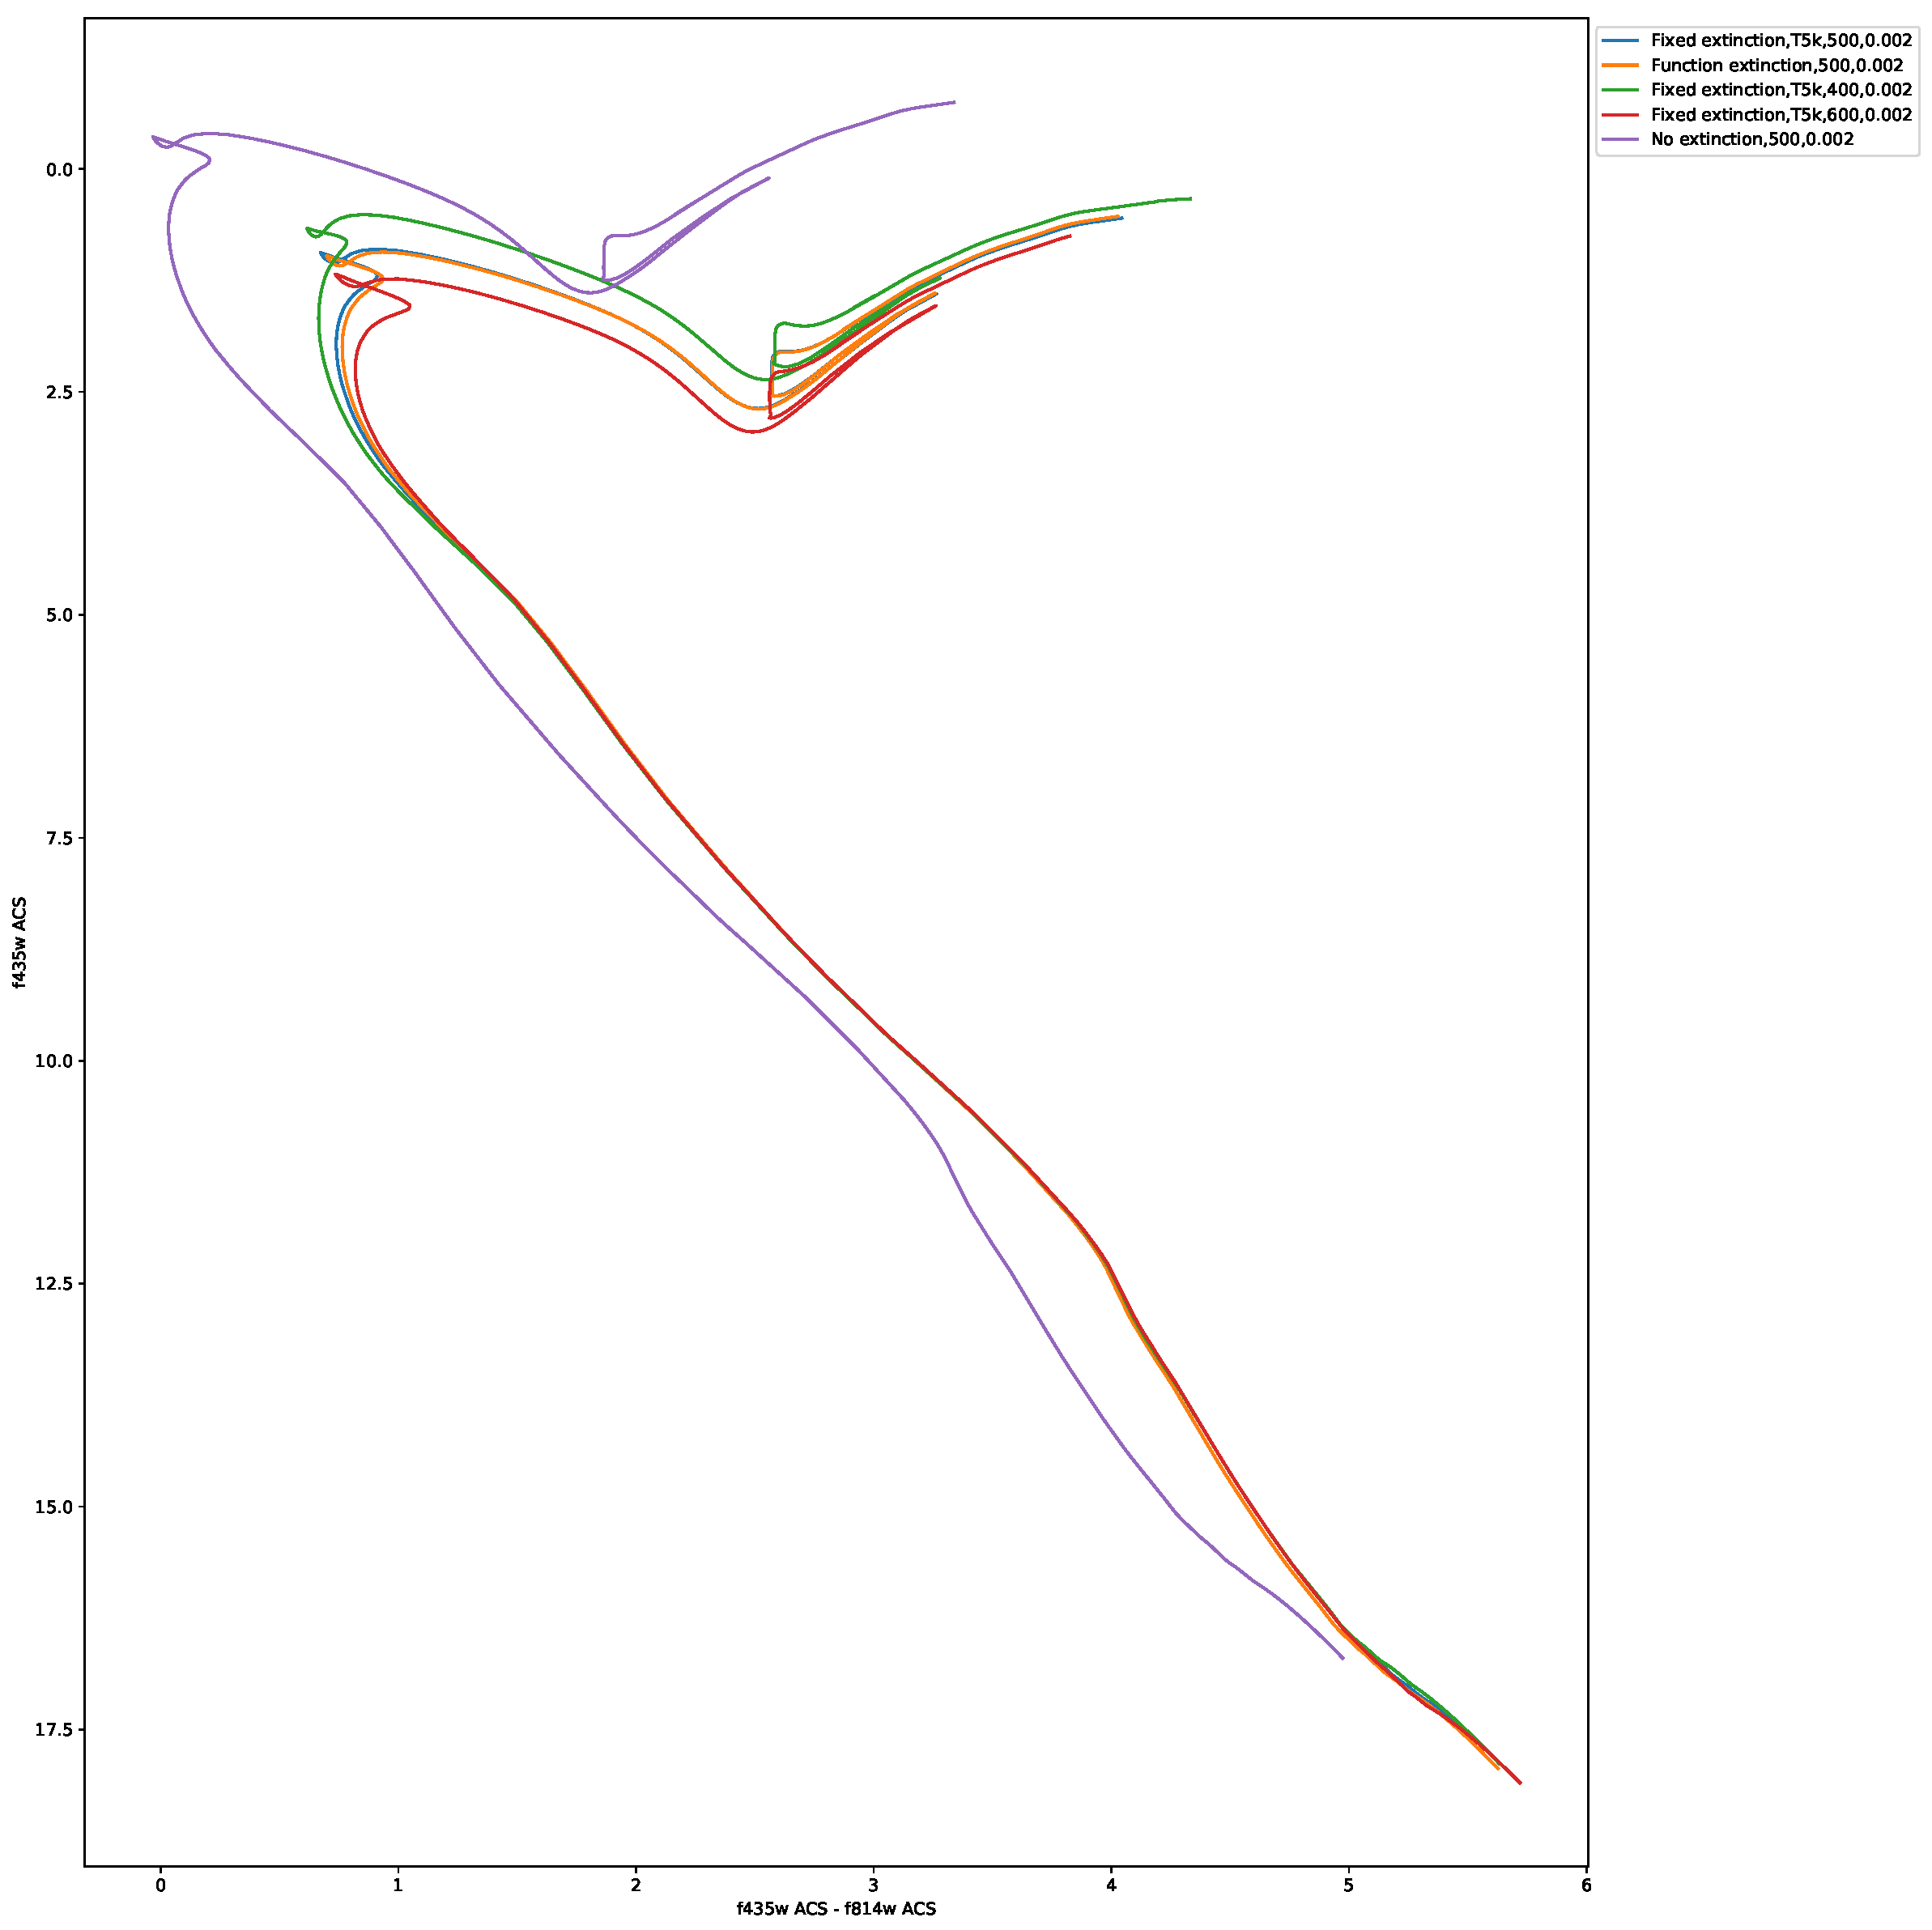
\includegraphics[scale=0.3]{../basti_isochrones_10_13Gyr/Extinction_T5k_FeH0fix_func_f435wACS_f435wACSmf814wACS_500_400_600_Myr_FeH_0p002_ref_noext_Av_1p0.pdf}
\caption{Ratios of $A_{X}/A_{V}$ values for different $Z$ values compared with solar metallicity data at log($g$) = 5.0}
\label{acs_isoc_T5k}
\end{center}
\end{figure}

\begin{figure}[h]
\begin{center}
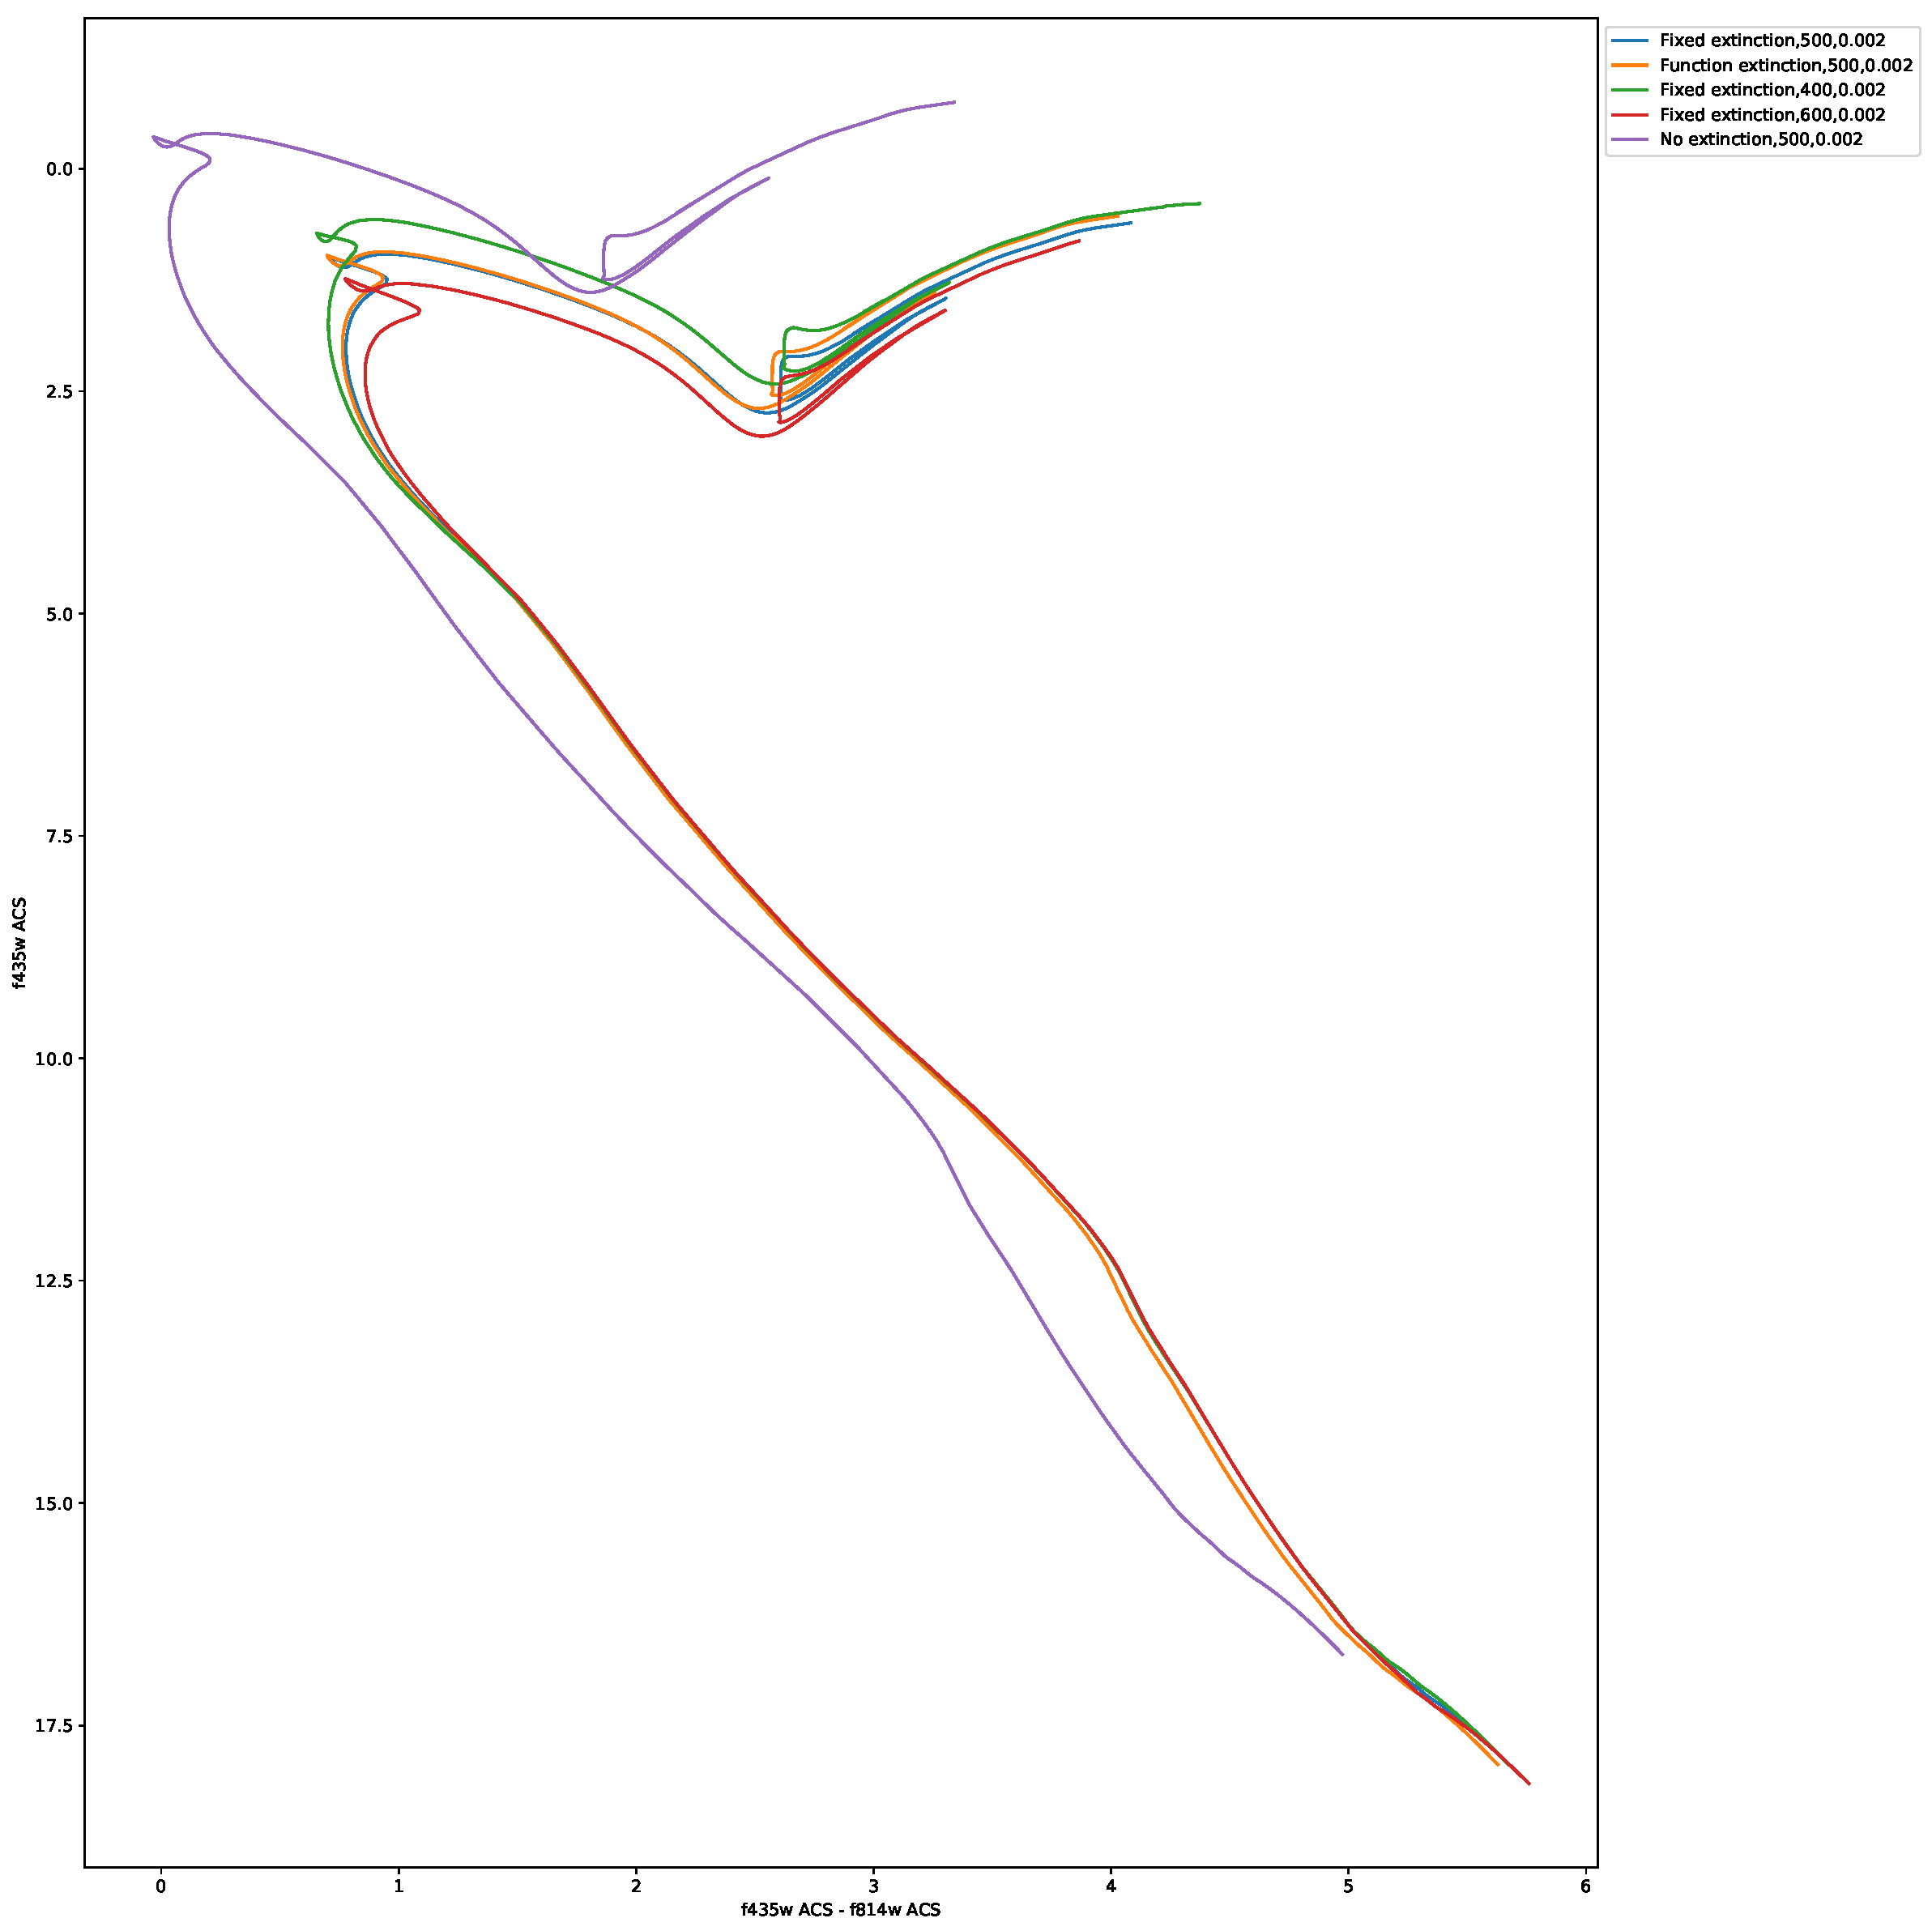
\includegraphics[scale=0.3]{../basti_isochrones_10_13Gyr/Extinction_T50k_FeH0fix_func_f435wACS_f435wACSmf814wACS_500_400_600_Myr_FeH_0p002_ref_noext_Av_1p0.pdf}
\caption{Ratios of $A_{X}/A_{V}$ values for different $Z$ values compared with solar metallicity data at log($g$) = 5.0}
\label{acs_isoc_T50k}
\end{center}
\end{figure}

\subsection{WFC3} \label{WFC3_isoc}

The CMD chosen for the ACS was the F435W-(F435W-F814W) axis combination. This CMD is useful as it pairs the bluest and reddest wide-field filters for the ACS, which produces larger spectral colours.****

\begin{figure}[h]
\begin{center}
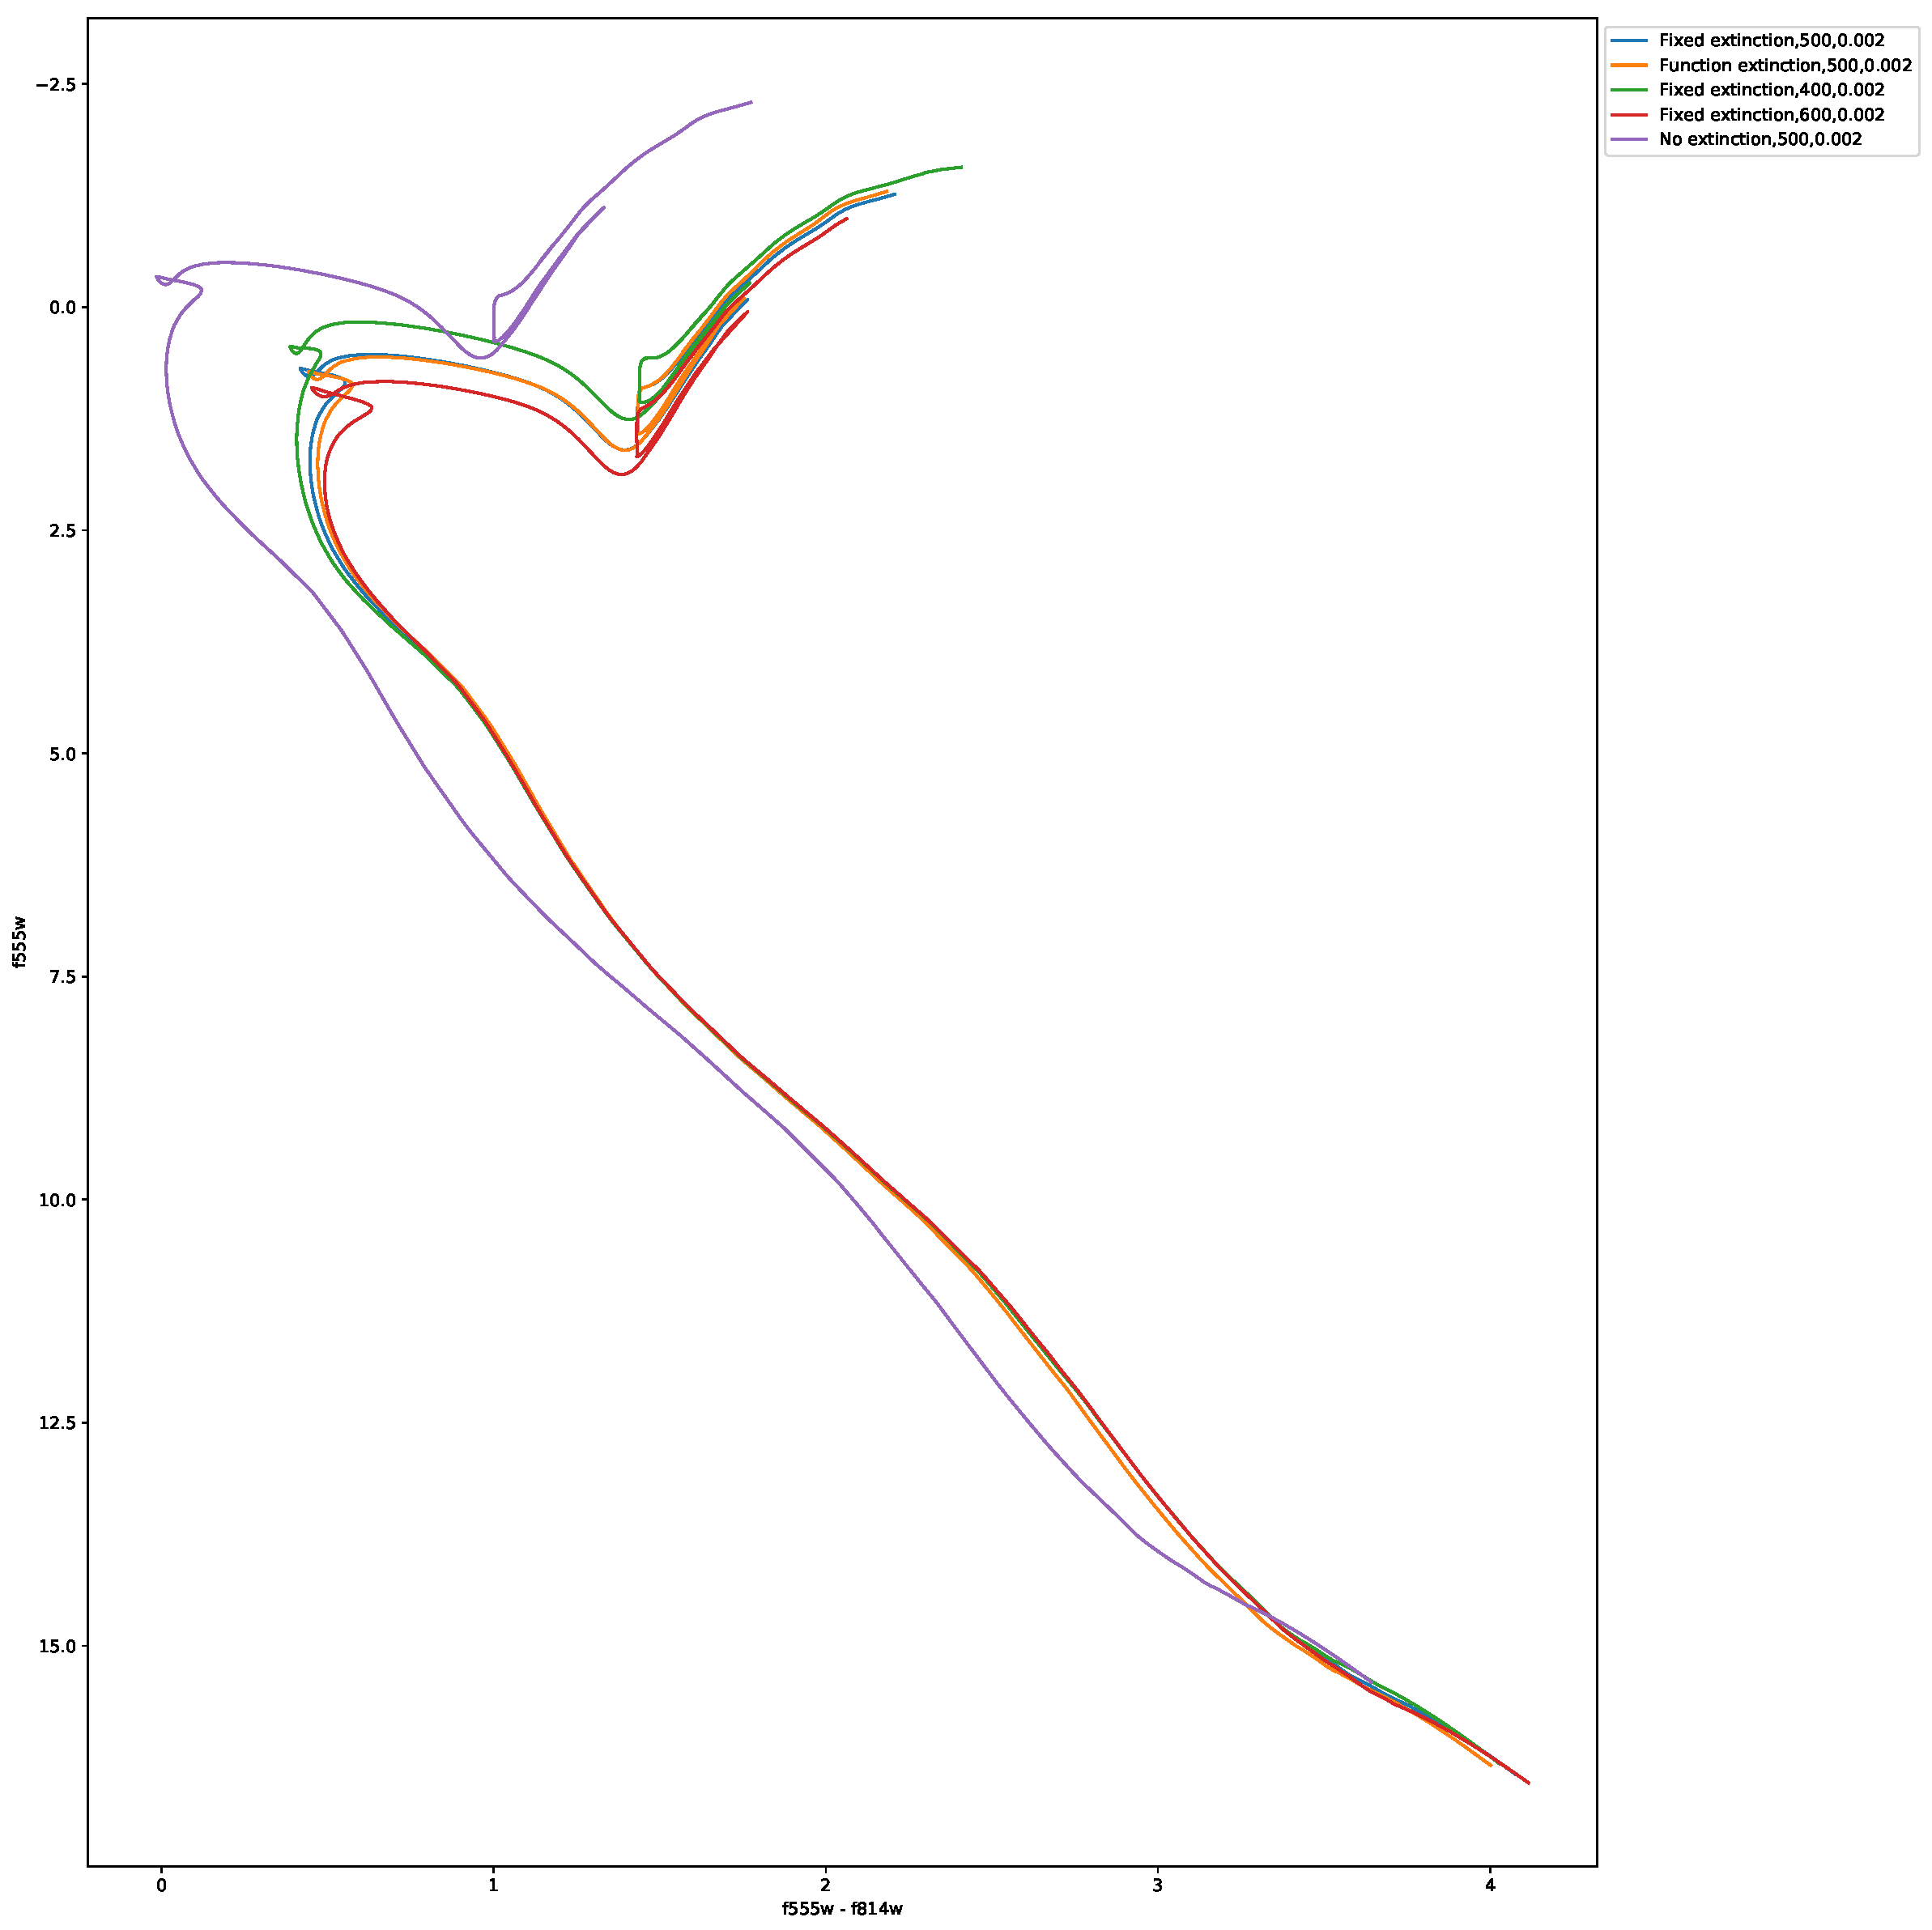
\includegraphics[scale=0.3]{../basti_isochrones_10_13Gyr/Extinction_T5k_FeH0fix_func_f555w_f555wmf814w_500_400_600_Myr_FeH_0p002_ref_noext_Av_1p0.pdf}
\caption{Ratios of $A_{X}/A_{V}$ values for different $Z$ values compared with solar metallicity data at log($g$) = 5.0}
\label{wfc3_isoc1_T5k}
\end{center}
\end{figure}

\begin{figure}[h]
\begin{center}
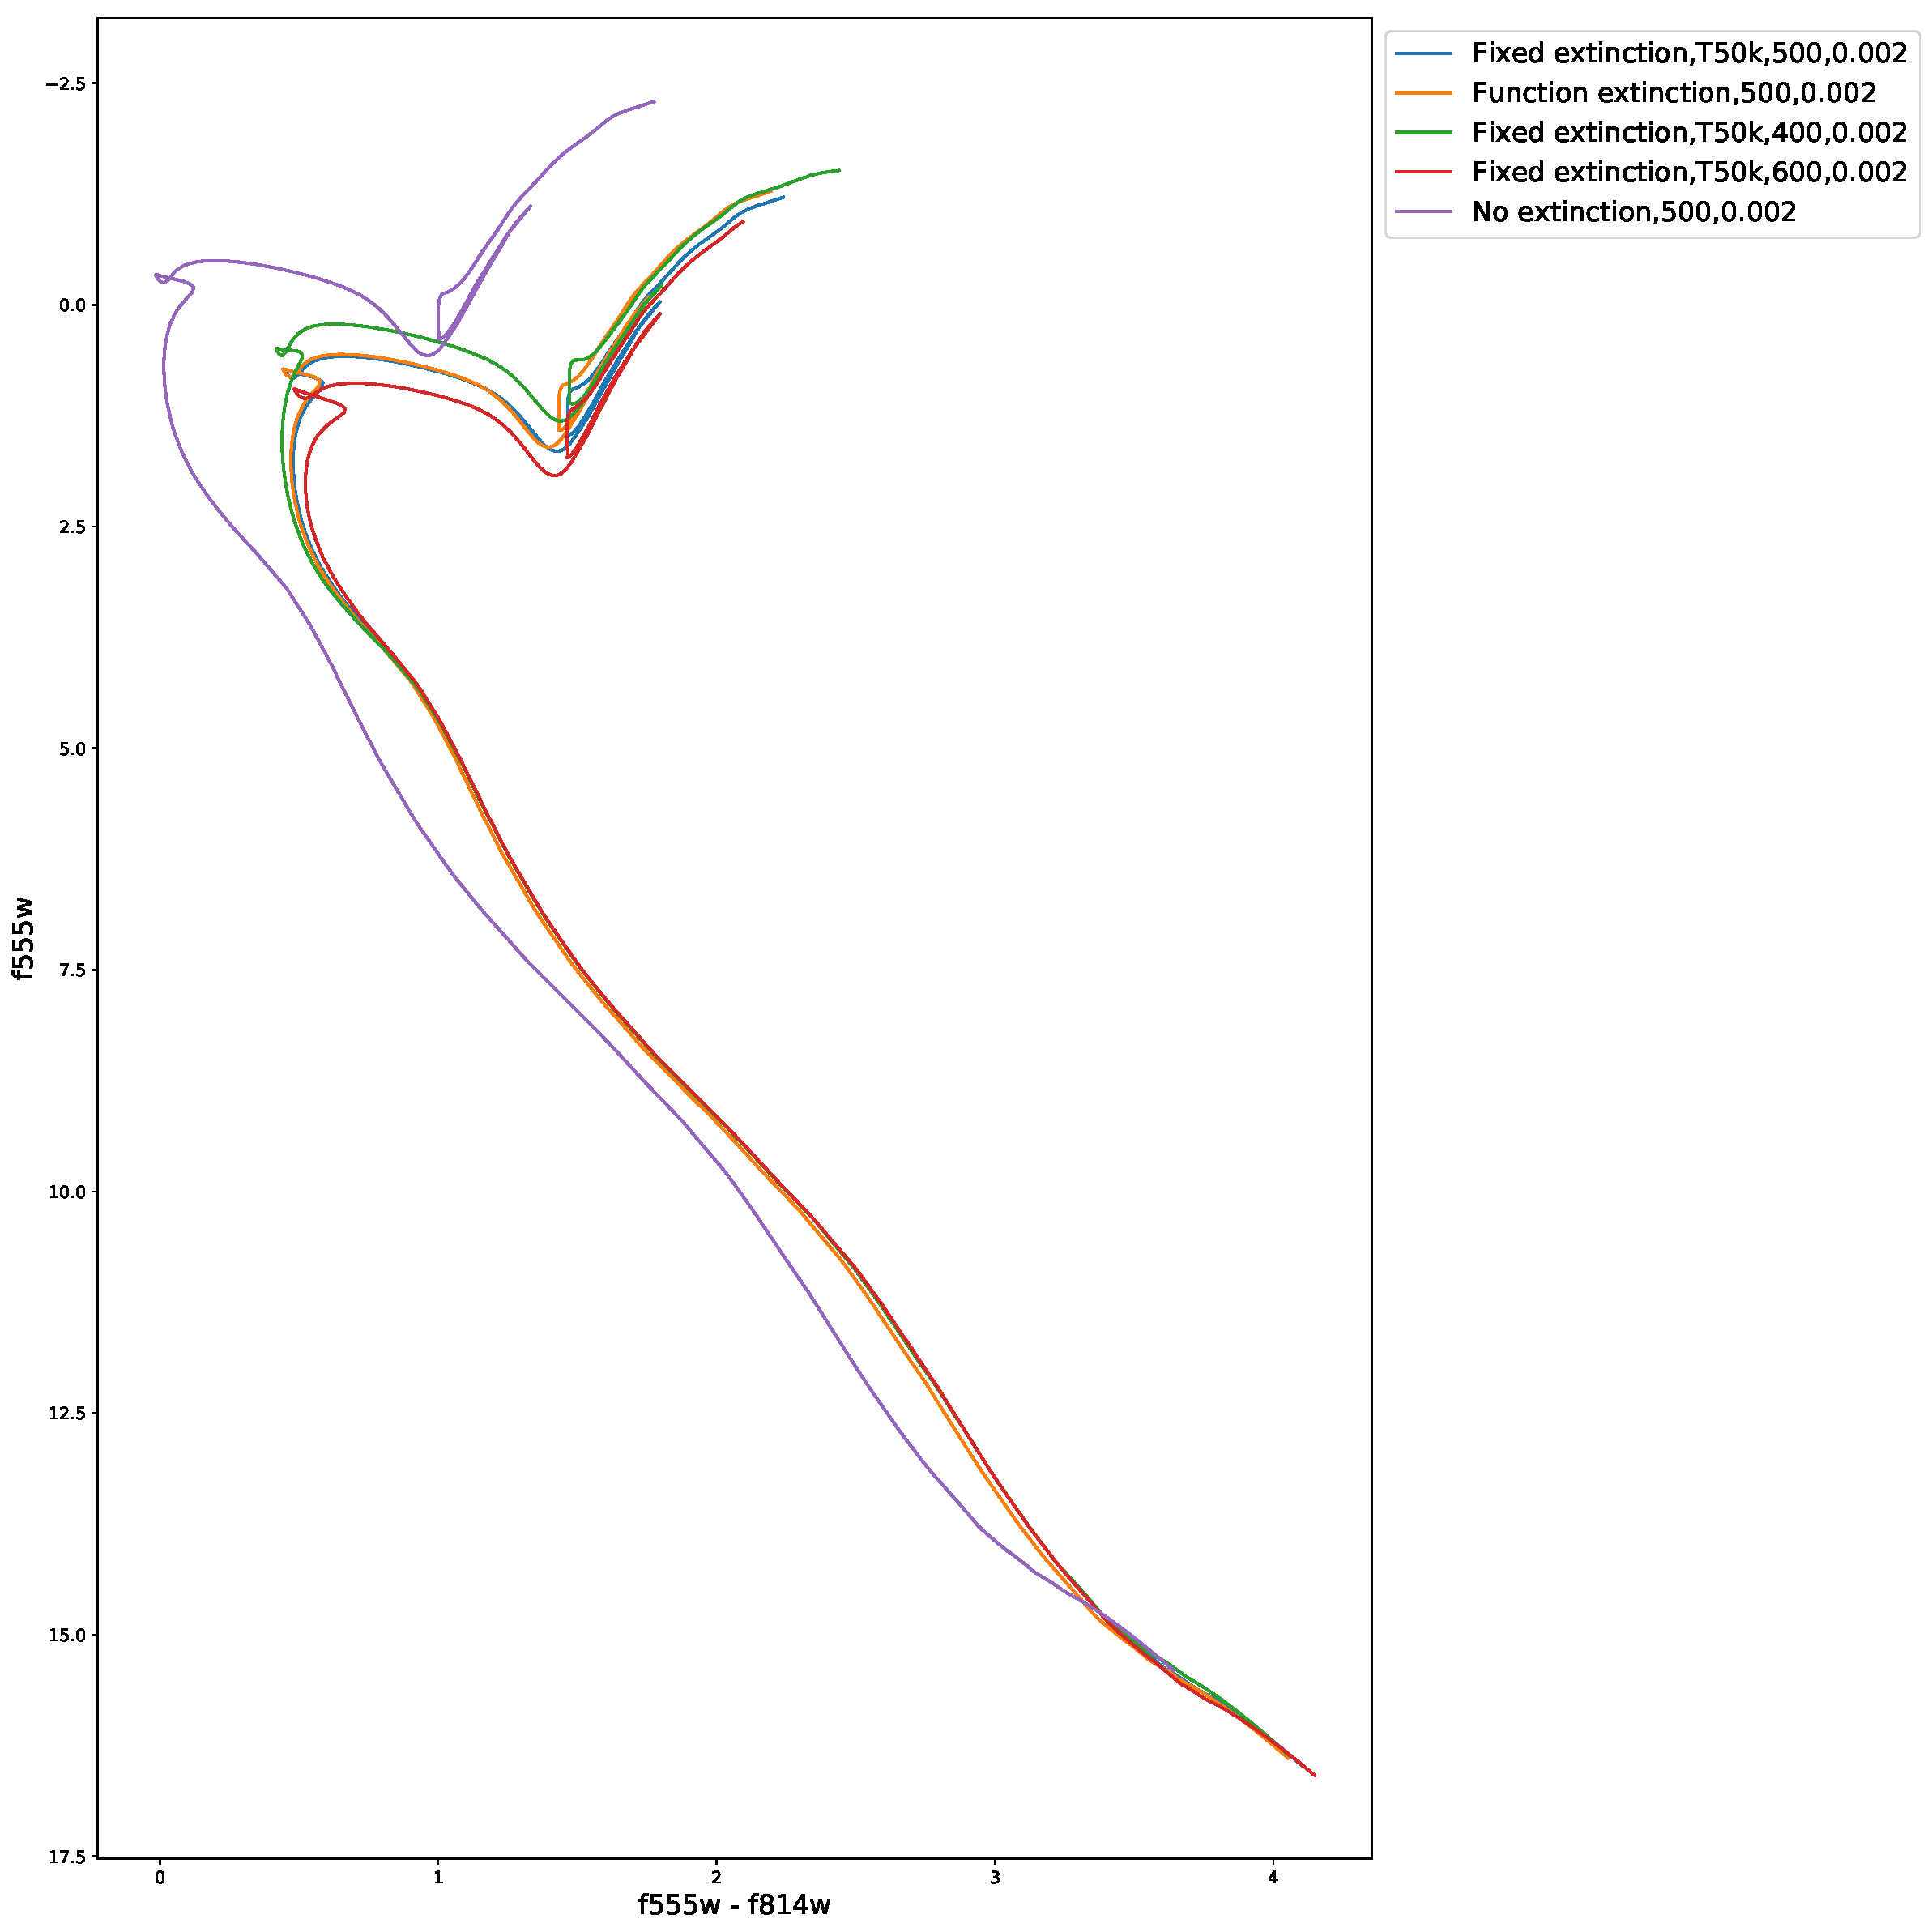
\includegraphics[scale=0.3]{../basti_isochrones_10_13Gyr/Extinction_T50k_FeH0fix_func_f555w_f555wmf814w_500_400_600_Myr_FeH_0p002_ref_noext_Av_1p0.pdf}
\caption{Ratios of $A_{X}/A_{V}$ values for different $Z$ values compared with solar metallicity data at log($g$) = 5.0}
\label{wfc3_isoc1_T50k}
\end{center}
\end{figure}

\begin{figure}[h]
\begin{center}
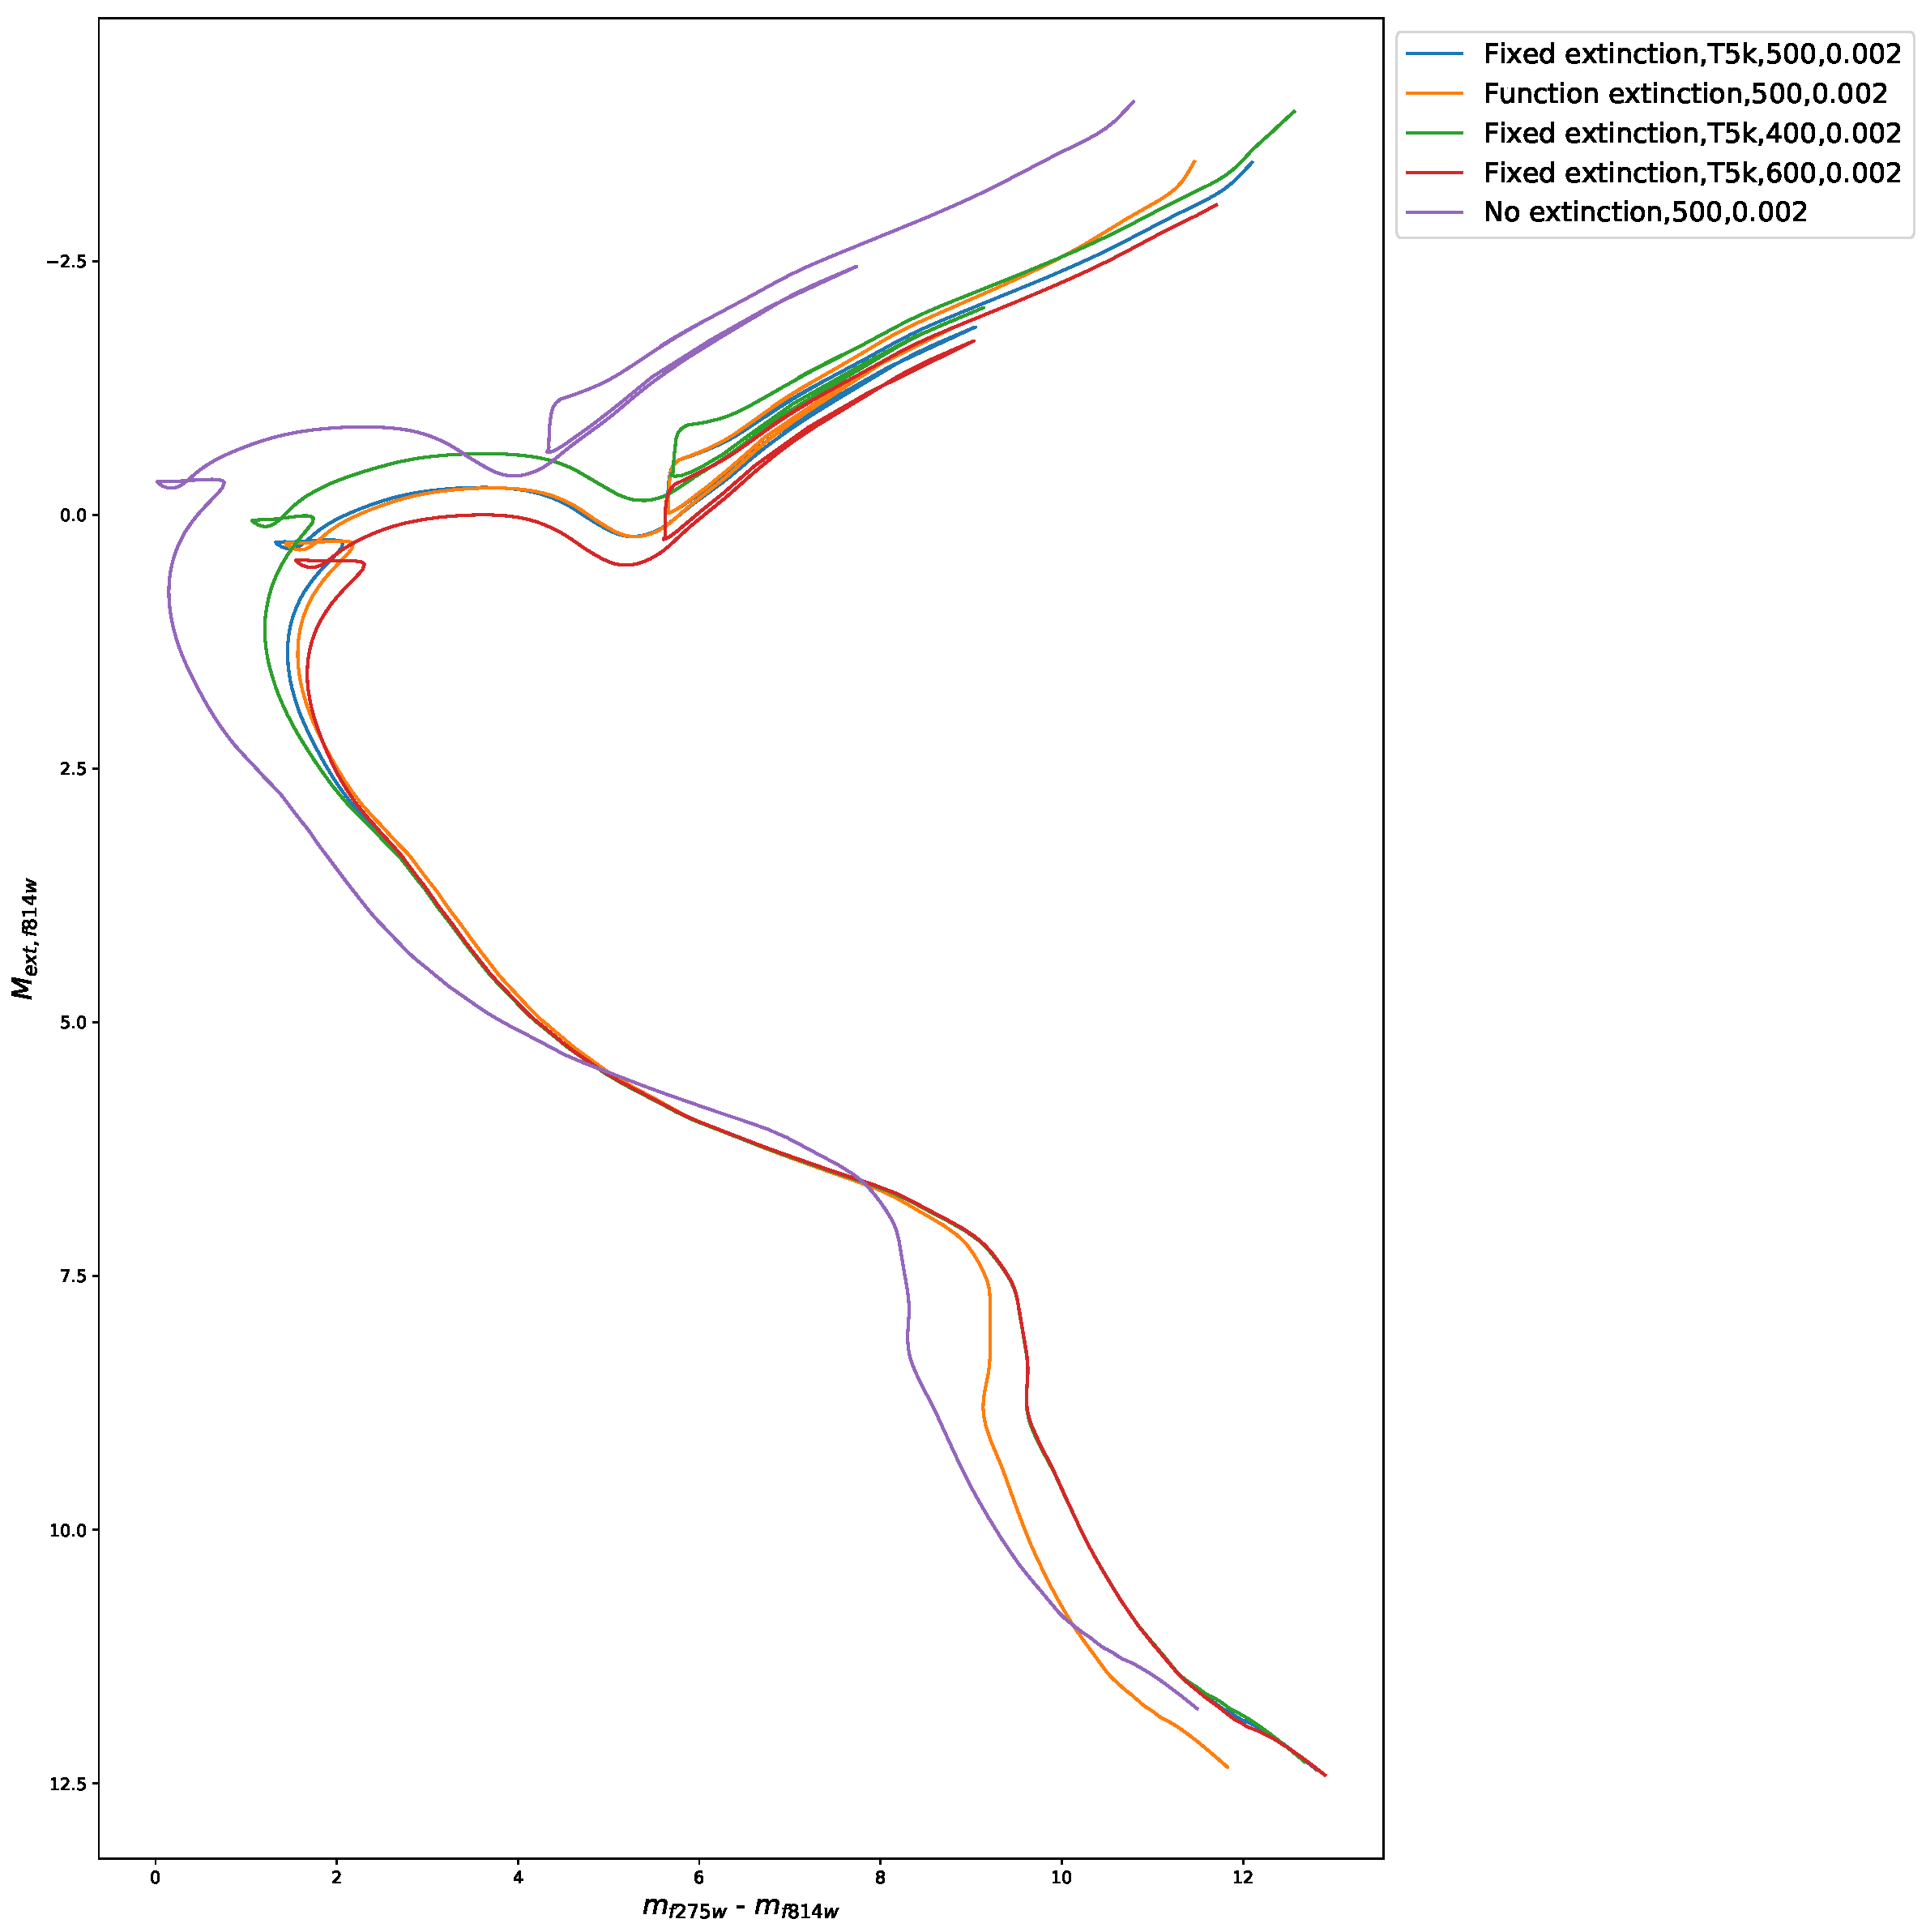
\includegraphics[scale=0.3]{../basti_isochrones_10_13Gyr/Extinction_T5k_FeH0fix_func_f814w_f275wmf814w_500_400_600_Myr_FeH_0p002_ref_noext_Av_1p0.pdf}
\caption{Ratios of $A_{X}/A_{V}$ values for different $Z$ values compared with solar metallicity data at log($g$) = 5.0}
\label{wfc3_isoc2_T5k}
\end{center}
\end{figure}

\begin{figure}[h]
\begin{center}
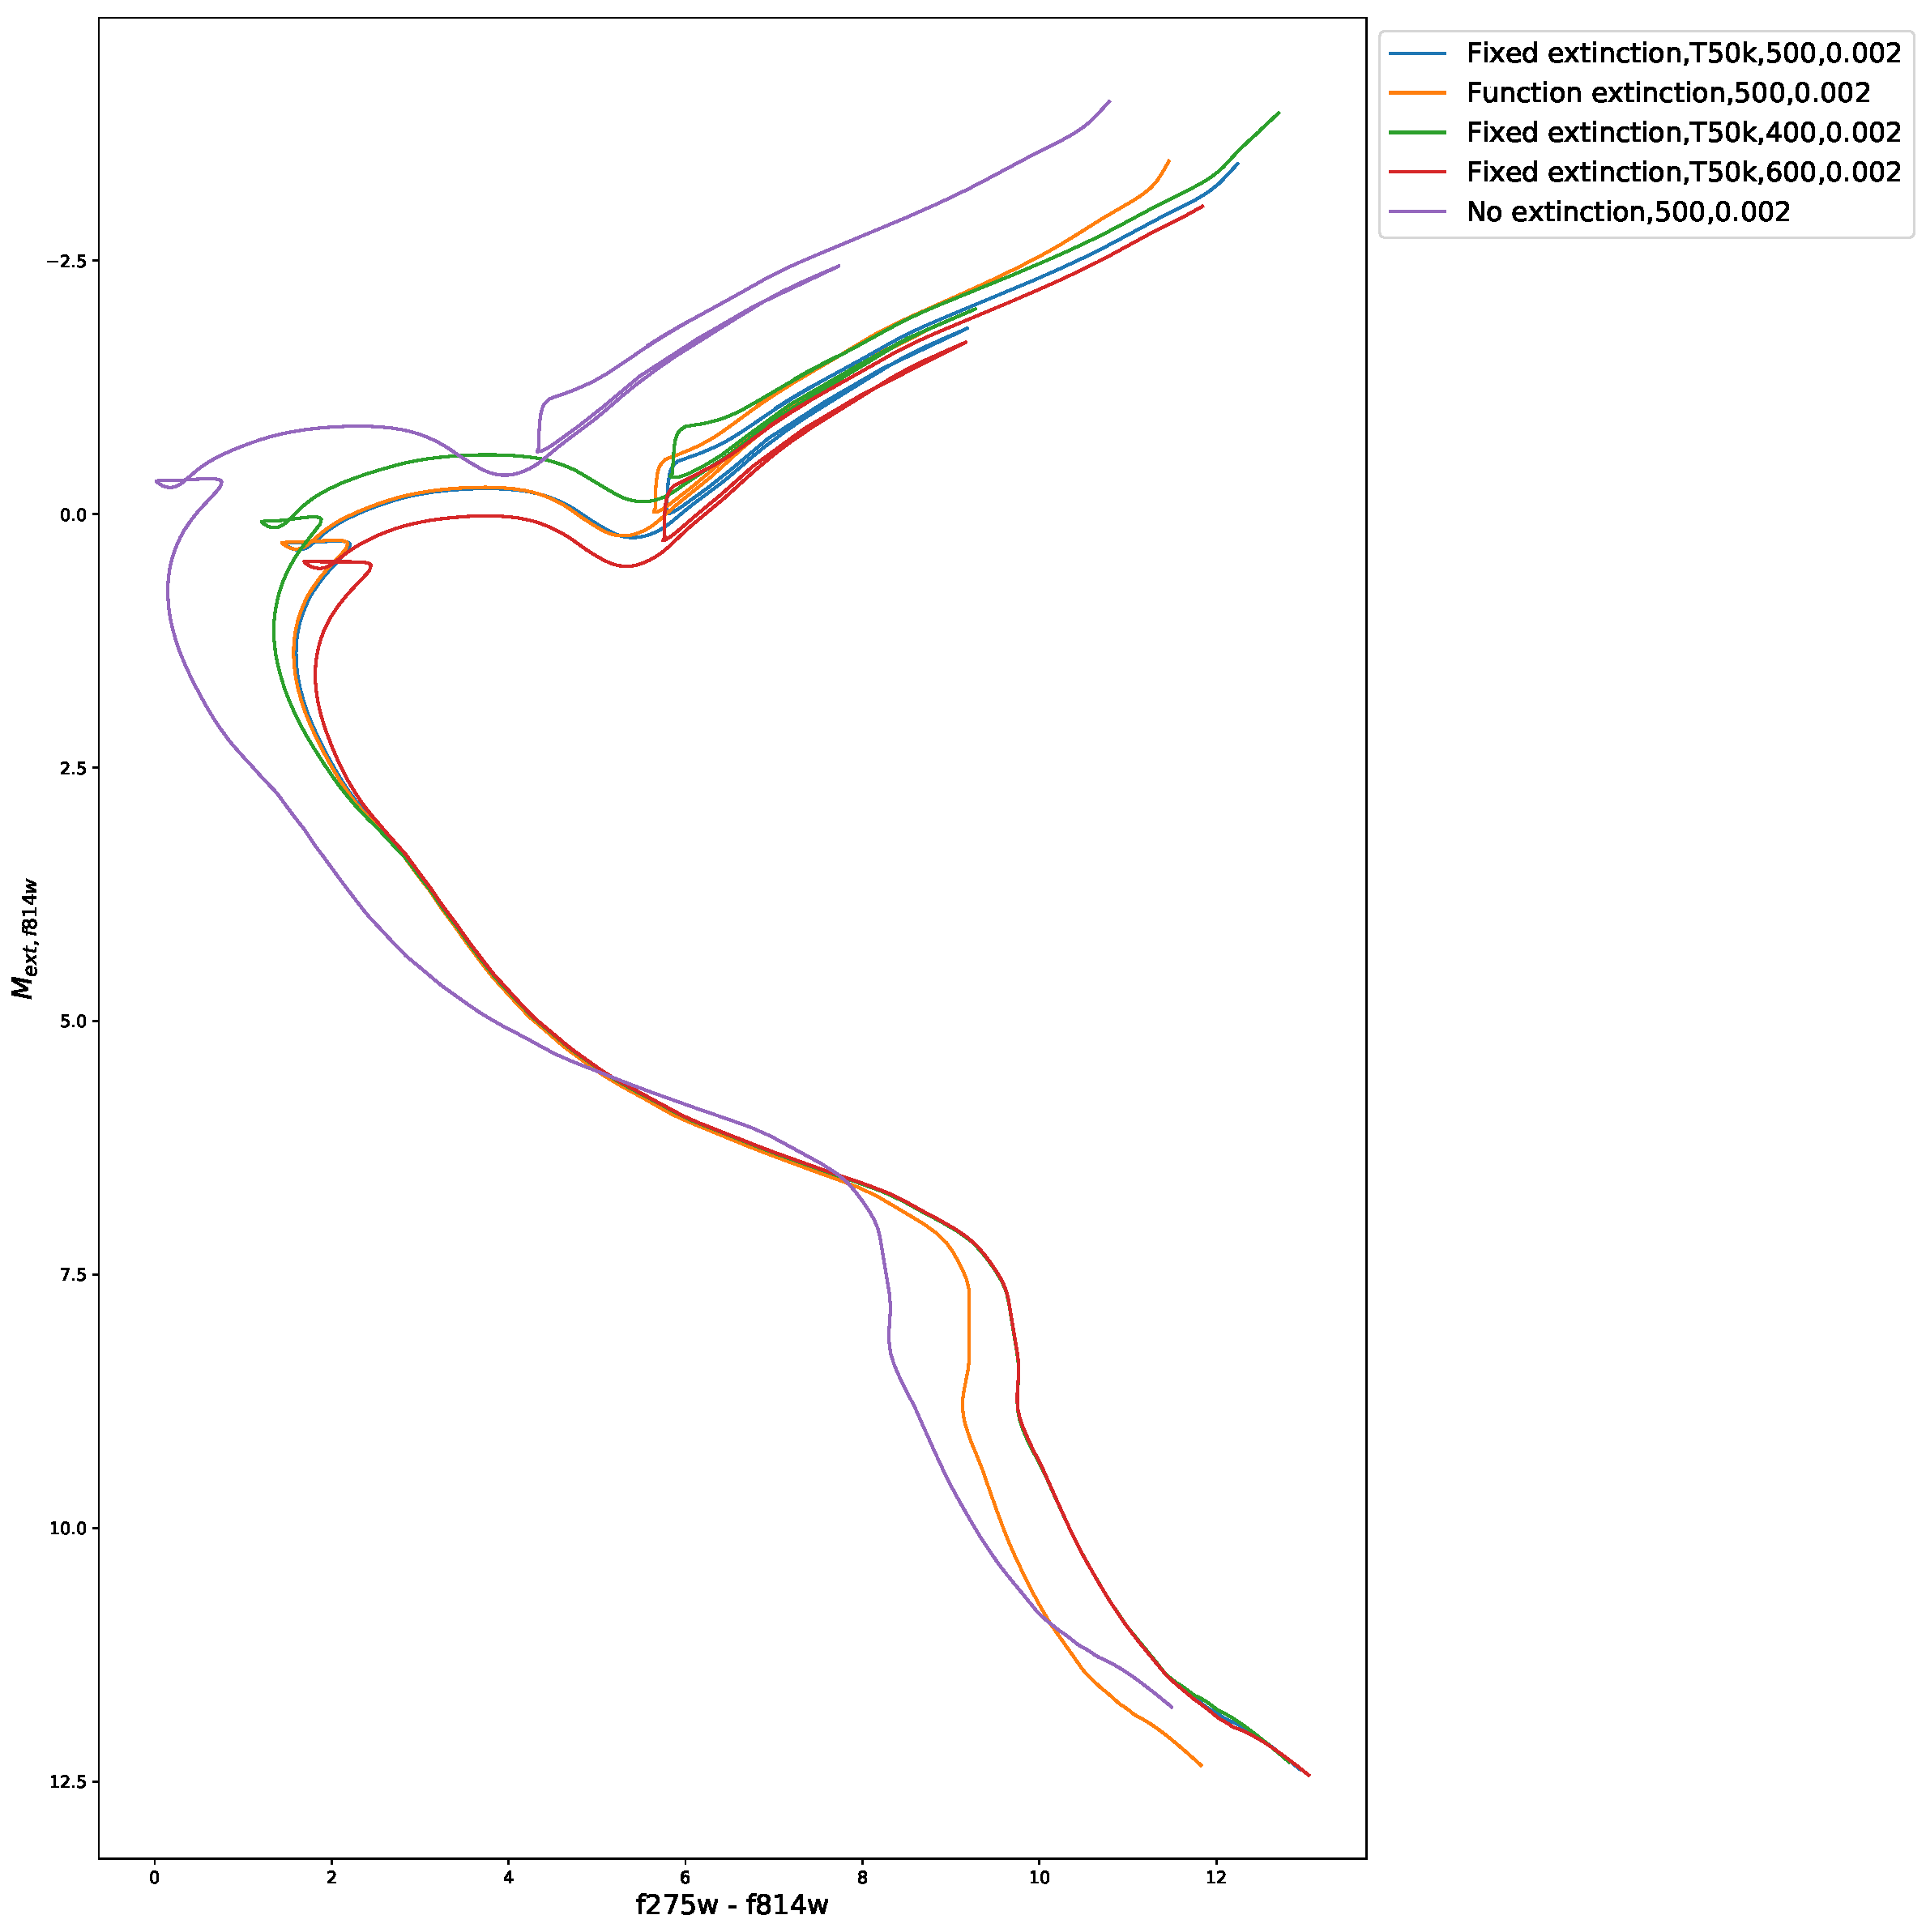
\includegraphics[scale=0.3]{../basti_isochrones_10_13Gyr/Extinction_T50k_FeH0fix_func_f814w_f275wmf814w_500_400_600_Myr_FeH_0p002_ref_noext_Av_1p0.pdf}
\caption{Ratios of $A_{X}/A_{V}$ values for different $Z$ values compared with solar metallicity data at log($g$) = 5.0}
\label{wfc3_isoc2_T50k}
\end{center}
\end{figure}

\subsection{Gaia} \label{Gaia_isoc}

Given that Gaia has only three photometric filters in total and given that the G\textsubscript{bp} and G\textsubscript{rp}  was the F435W-(F435W-F814W) axis combination. This CMD is useful as it pairs the bluest and reddest wide-field filters for the ACS, which produces larger spectral colours.****

\begin{figure}[h]
\begin{center}
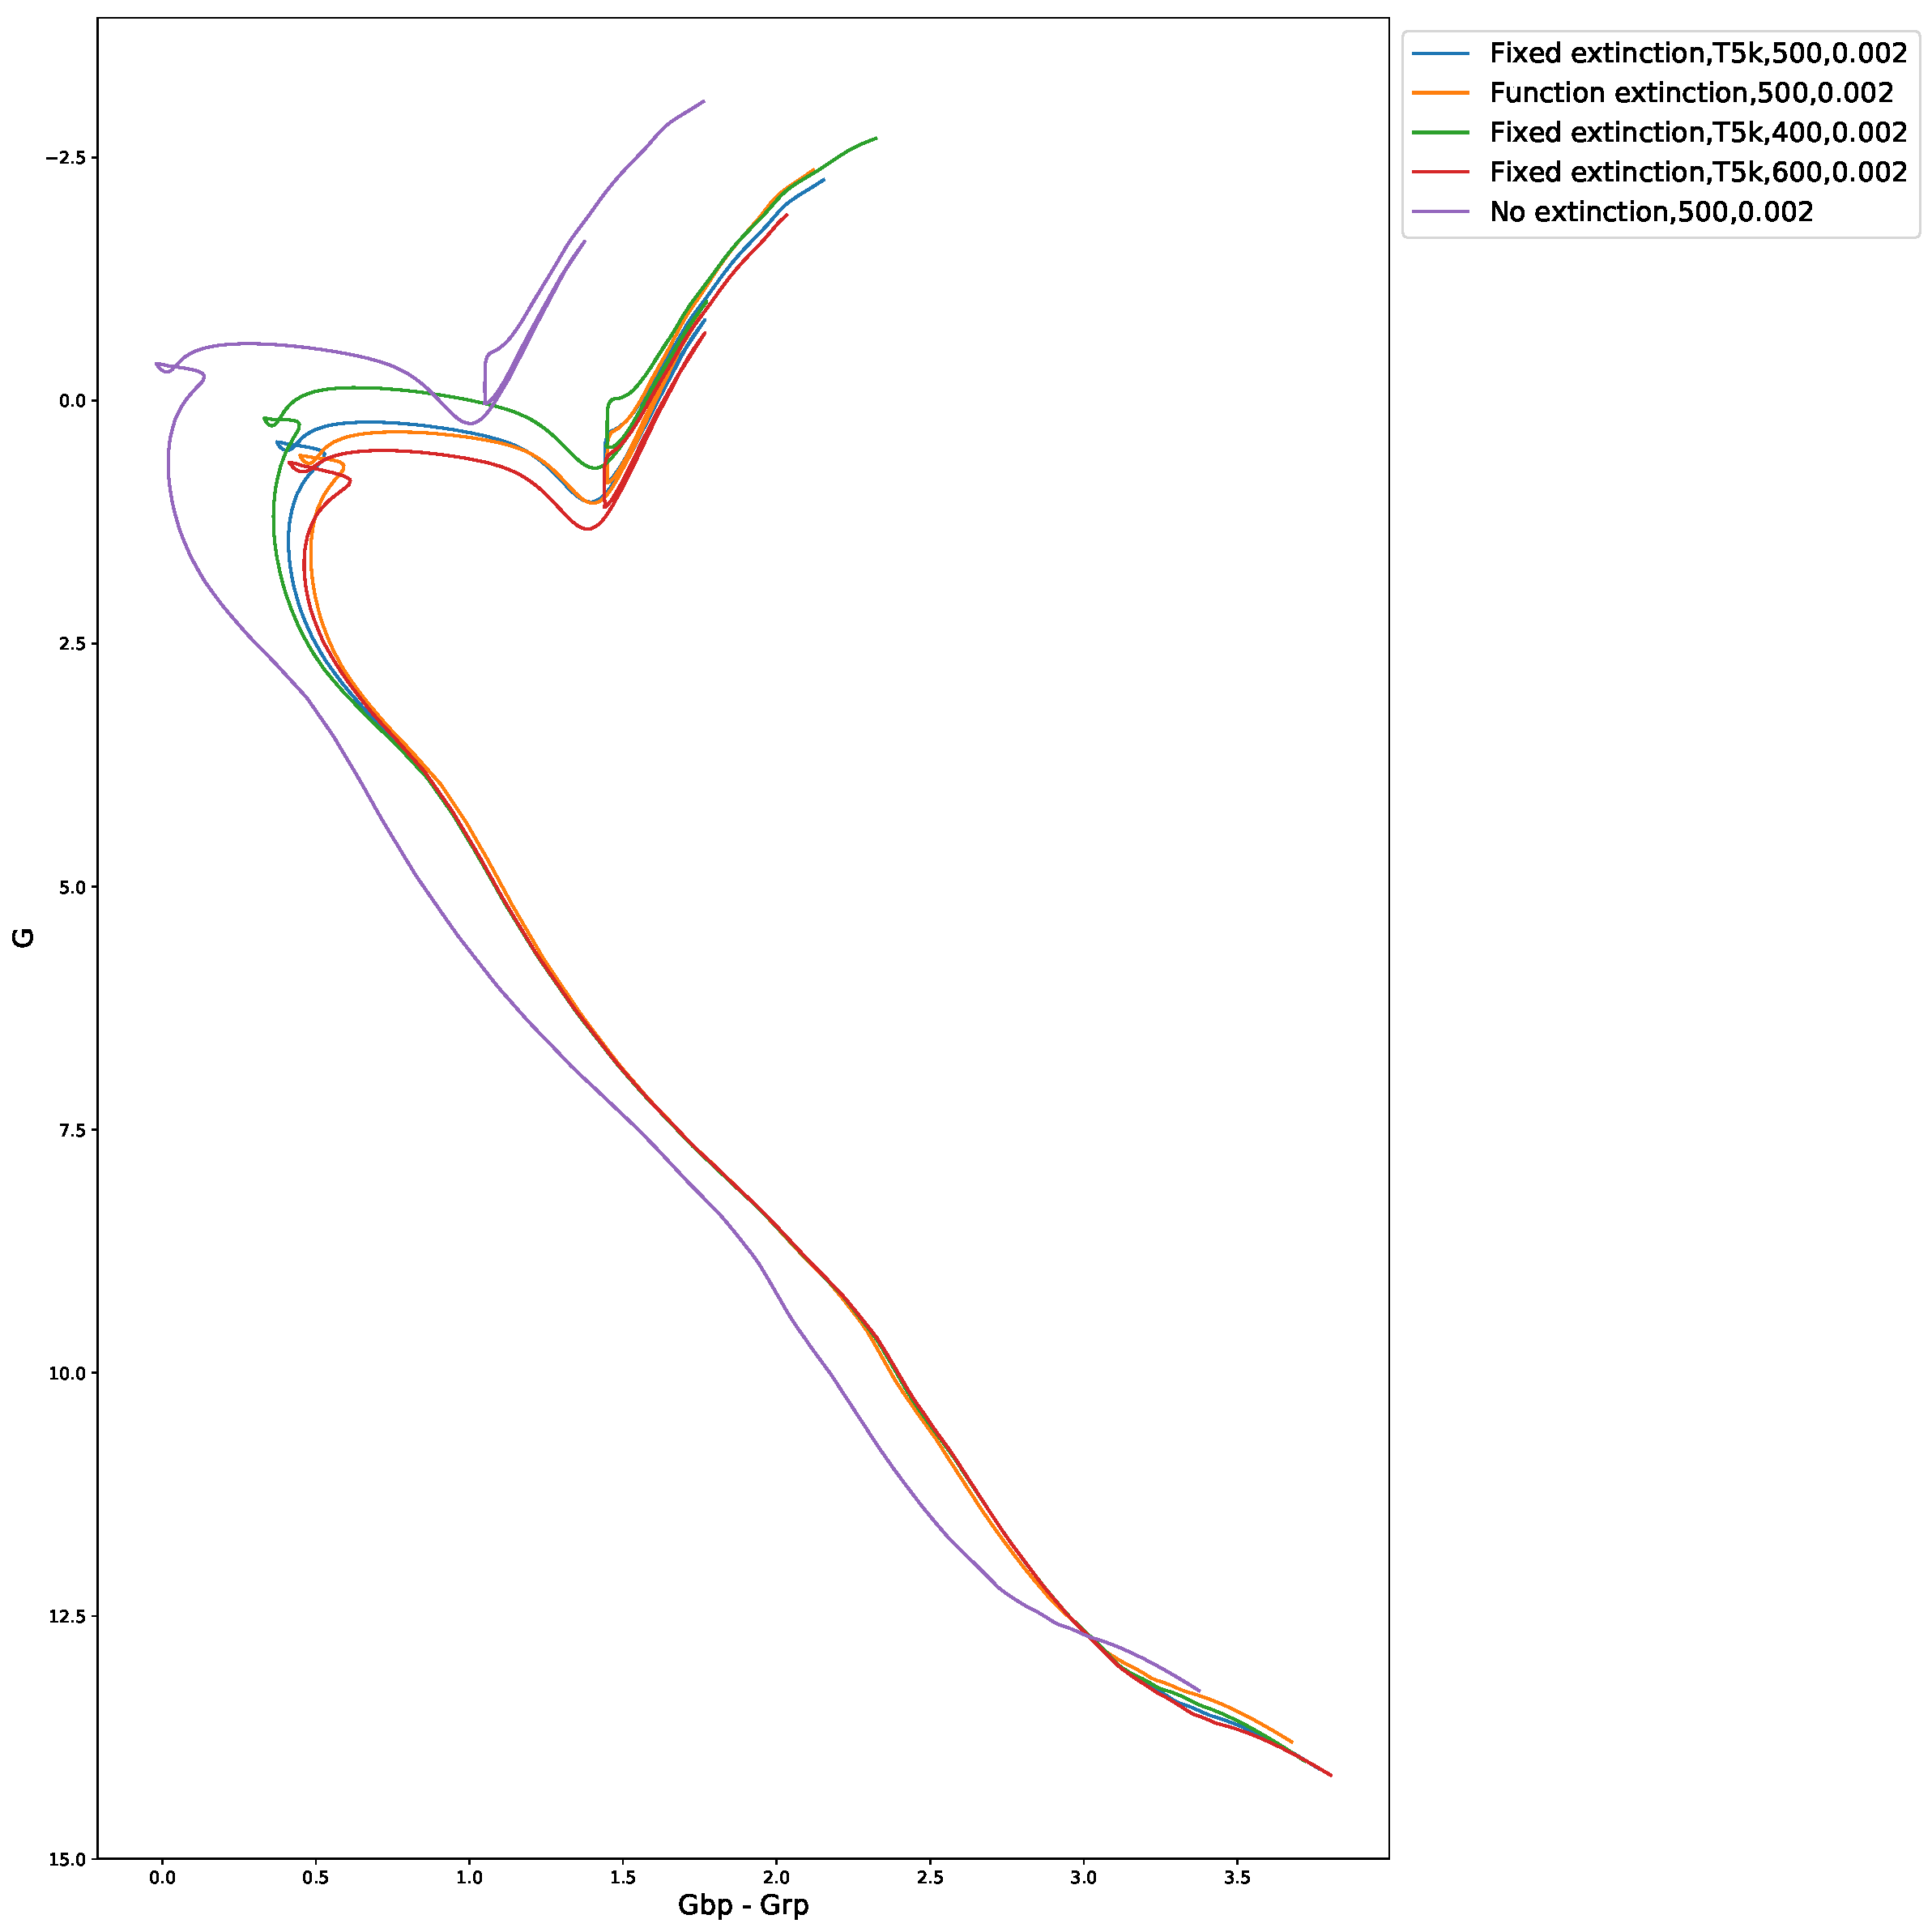
\includegraphics[scale=0.3]{../basti_isochrones_10_13Gyr/Extinction_T5k_FeH0fix_func_G_GbpmGrp_500_400_600_Myr_FeH_0p002_ref_noext_Av_1p0.pdf}
\caption{Ratios of $A_{X}/A_{V}$ values for different $Z$ values compared with solar metallicity data at log($g$) = 5.0}
\label{gaia_isoc_T5k}
\end{center}
\end{figure}

\begin{figure}[h]
\begin{center}
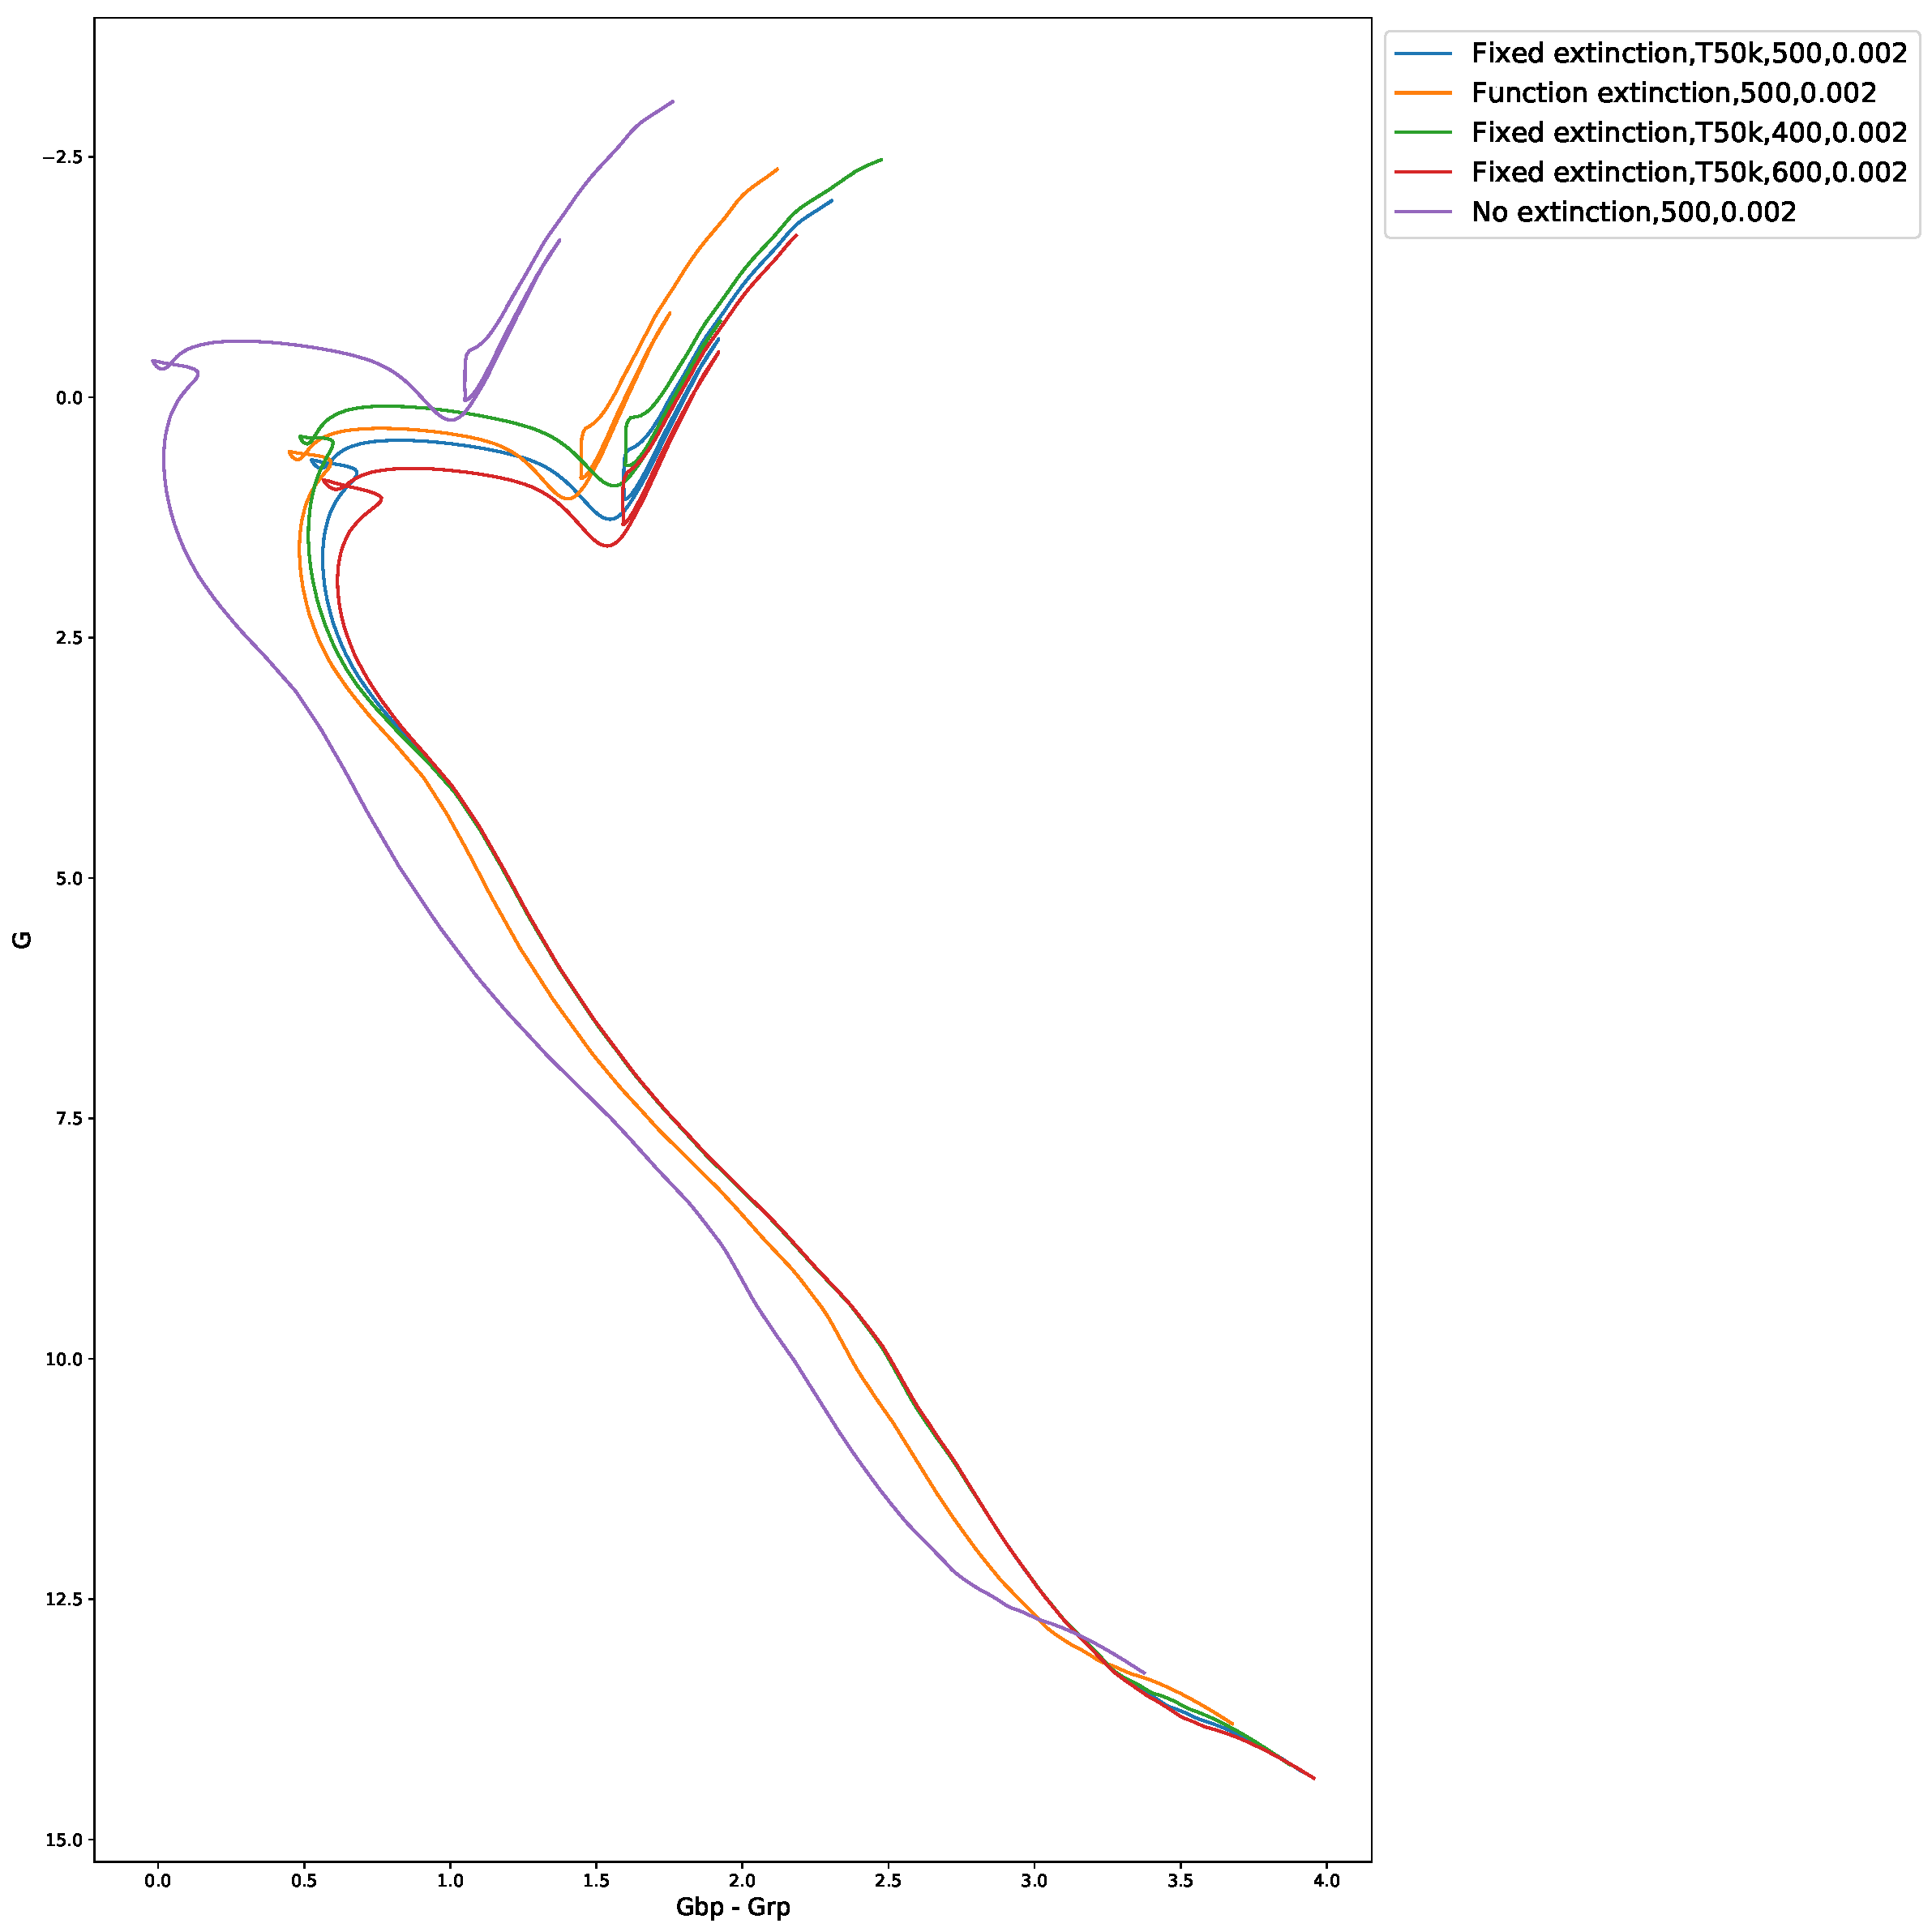
\includegraphics[scale=0.3]{../basti_isochrones_10_13Gyr/Extinction_T50k_FeH0fix_func_G_GbpmGrp_500_400_600_Myr_FeH_0p002_ref_noext_Av_1p0.pdf}
\caption{Ratios of $A_{X}/A_{V}$ values for different $Z$ values compared with solar metallicity data at log($g$) = 5.0}
\label{gaia_isoc_T50k}
\end{center}
\end{figure}

\section{Test case: NGC 6793}
To test the effects of the difference in treatment of $A_{X}/A{V}$, both cases were employed to predict the isochrone ***parameters of the open cluster NGC 6793.

\subsection{Observational background}
NGC 6793 has little information available compared to many other open clusters. Two estimates for observational properties of the cluster have been published and are listed in Table \ref{NGC6793_obs}.

\begin{table}
\begin{center}
\begin{tabular}{ccc}
\hline
%\multirow{2}{*}{System} & \multirow{2}{*}{Filter} & \multirow{2}{*}{$A_{1}$ function} & \multicolumn{3}{c}{$A_{1}$ coefficients} \\ \cline{4-6}
%\textbf{Filter} \\
Cluster property & K05 & GC18 \\
\hline
Distance modulus / mag & 10.73 & 8.894 \\
-> distance / pc & 1400 & 601 \\
log(age / yr) & 8.64 & 8.78 \\
-> Age / Myr & 437 & 603 \\
$E(B-V)$ / mag & 0.17 & 0.272 \\
$[Fe/H]$ & ? & ? \\
Members & ? (> 3 ACSS-2.5) & 465 (271 with Gaia photometry) \\
\hline
\end{tabular}
\caption{Observational parameters for NGC 6793, according to \cite{2005A&A...438.1163K} (WEBDA archive page) and \cite{2018A&A...616A..10G}}
\label{NGC6793_obs}
\end{center}
\end{table}

\subsection{Comparison of extinction methods}
The Gaia DR2 dataset, containing the parallaxes and apparent magnitudes (in all three Gaia filters) for 338 objects tagged as belonging to NGC 6793, was obtained. The number of objects is greater than the 271 photometric Gaia objects found by \cite{2018A&A...616A..10G}. There were significant variations in the observed parallaxes of individual stars, far beyond the maximum cluster radii expected (\cite{2006A&A...456..523S} - general open cluster properties).

There are highly significant errors for the individual objects in the Gaia data propagation, even when assuming the only source of error is from  parallax measurements (see Figure \ref{ngc_errorbars}). The magnitude of the errorbars dwarf any changes in isochrones due to extinction coefficient treatments.

All, as shown in Section****, the isochrones are sensitive both to the reference extinction coefficient value $A_{V}$ and to the value of $A_{X}/A_{V}$ for the fixed case. Some individual parts of the isochrones relevant to this study are additionally sensitive to other isochrone parameters:

\begin{enumerate}
%, but metallicity has a smaller effect
\item The position of the MSTO is sensitive to the treatment of $A_{X}/A_{V}$, as shown in Section****, and the isochrone age.
\item The position of the lower main sequence is significantly more sensitive to metallicity than other parts of the isochrone.
\end{enumerate}



\begin{figure}[h]
\begin{center}
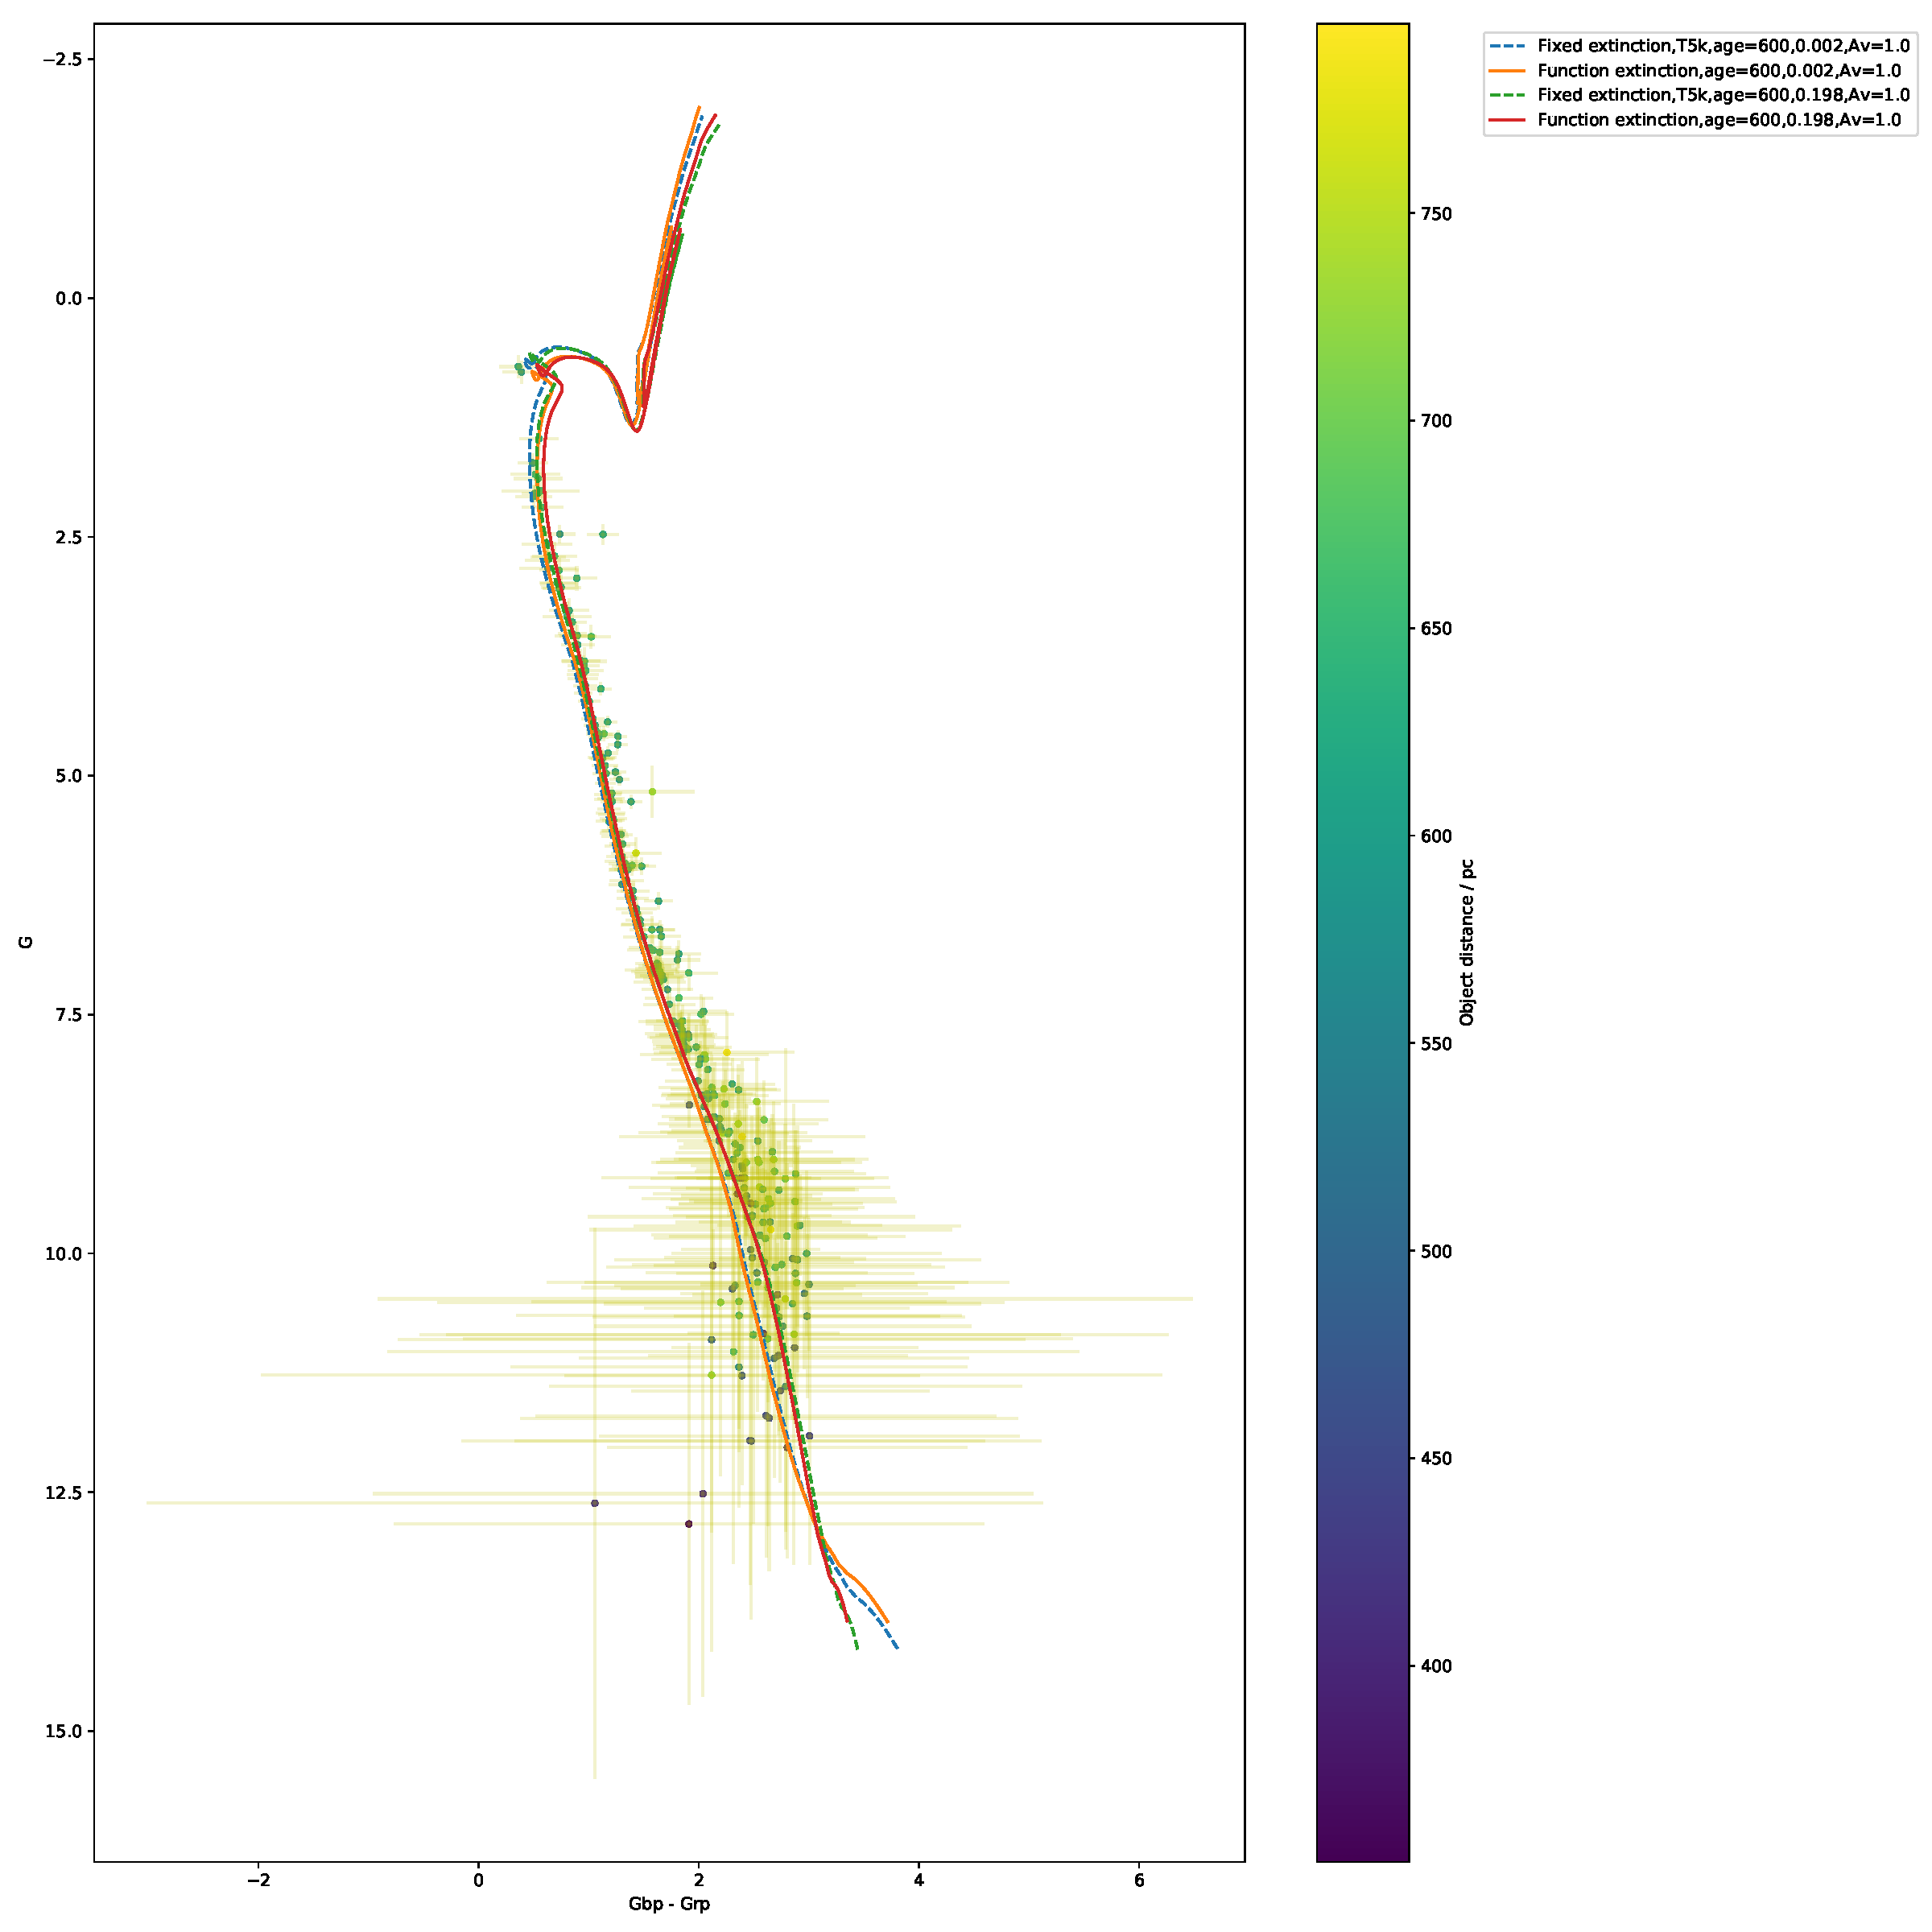
\includegraphics[scale=0.3]{../NGC_6793_CMD_FeH_0p002_0p198_Av_1p0_600Myr_isochrones_both_errorbars_T5k.pdf}
\caption{Gaia CMD of NGC 6793 with errorbars included.}
\label{ngc_errorbars}
\end{center}
\end{figure}

\chapter{Conclusion}
In all cases, applying a fixed extinction to all points in an isochrone causes the main-sequence turn-off to occur at a more luminous, bluer point in a given CMD than the MSTO point for an extinction coefficient described using a function fitted to empirically derived data.

\section{Future work}


\bibliographystyle{mnras} % unsrtnat
\bibliography{mphil_thesis}

\end{document}